\pdfoutput=1

\documentclass{l4proj}

%
% put any packages here
%
\usepackage{mathtools}
\usepackage{amsmath}
\usepackage{amssymb}
\usepackage{amsthm}
\usepackage{subcaption}
\usepackage{float}
\usepackage{array,multirow}
\usepackage{url}
\usepackage{hyperref}
\usepackage[table]{xcolor}
\usepackage{array}
\usepackage{booktabs}
\usepackage[toc,page]{appendix}
\usepackage[utf8]{inputenc}
\usepackage[acronym]{glossaries}

\usepackage{algorithm}
\usepackage{algpseudocode}
%\PassOptionsToPackage{noend}{algpseudocode}% comment out if want end's to show
\makeatletter
\def\BState{\State\hskip-\ALG@thistlm}
%\makeatother

% start with some helper code
% This is the vertical rule that is inserted
\newcommand*{\algrule}[1][\algorithmicindent]{\makebox[#1][l]{\hspace*{.5em}\vrule height .75\baselineskip depth .25\baselineskip}}%

\newcount\ALG@printindent@tempcnta
\def\ALG@printindent{%
    \ifnum \theALG@nested>0% is there anything to print
        \ifx\ALG@text\ALG@x@notext% is this an end group without any text?
            % do nothing
            \addvspace{-3pt}% FUDGE for cases where no text is shown, to make the rules line up
        \else
            \unskip
            % draw a rule for each indent level
            \ALG@printindent@tempcnta=1
            \loop
                \algrule[\csname ALG@ind@\the\ALG@printindent@tempcnta\endcsname]%
                \advance \ALG@printindent@tempcnta 1
            \ifnum \ALG@printindent@tempcnta<\numexpr\theALG@nested+1\relax% can't do <=, so add one to RHS and use < instead
            \repeat
        \fi
    \fi
    }%
\usepackage{etoolbox}
% the following line injects our new indent handling code in place of the default spacing
\patchcmd{\ALG@doentity}{\noindent\hskip\ALG@tlm}{\ALG@printindent}{}{\errmessage{failed to patch}}
\makeatother



\makeglossaries
\glstoctrue
\definecolor{Gray}{gray}{0.85}

\newcounter{example}[section]
\newenvironment{example}[1][]{\refstepcounter{example}\par\medskip
   \noindent \textit{Example~\theexample #1} \rmfamily}{\medskip}
\newtheorem{theorem}{Theorem}[section]
\newtheorem{lemma}[theorem]{Lemma}
\newtheorem{proposition}[theorem]{Proposition}
\newtheorem{corollary}[theorem]{Corollary}
\newtheorem{definition}{Definition}

\newcommand{\Lagr}{\mathcal{L}}
\newcommand{\fancyA}{\mathcal{A}}
\newcommand{\fancyI}{\mathcal{I}}
\newcommand{\fancyC}{\mathcal{C}}
\newcommand{\fancyP}{\mathcal{P}}
%%%%%%%%% glossary entries and acronyms %%%%%%%%%%%%%%%%%%%%

%%% The glossary entry the acronym links to   
\newglossaryentry{apig}{name={API},
    description={An Application Programming Interface (API) is a particular set
of rules and specifications that a software program can follow to access and
make use of the services and resources provided by another particular software
program that implements that API}}
%%%%%%%%%%%
%%% define the acronym and use the see= option
\newglossaryentry{api}{name={API}, description={Application
Programming Interface}, first={Application
Programming Interface (API)\glsadd{apig}}, see=[Glossary:]{apig}}
%
\newglossaryentry{sip}{type=\acronymtype, name={SIP}, description={subgraph isomorphism problem}, first={Subgraph Isomorphism Problem (SIP)}}
%
\newglossaryentry{sat}{type=\acronymtype, name={SAT}, description={Satisfiable}, first={satisfiable (SAT)}}
%
\newglossaryentry{unsat}{type=\acronymtype, name={UNSAT}, description={Unsatisfiable}, first={unsatisfiable (UNSAT)}}
%
\newglossaryentry{graph}{type=\acronymtype, name={G}, description={graph}, first={graph (G)}}
%
\newglossaryentry{target}{type=\acronymtype, name={G$_{t}$}, description={target graph}, first={target (G$_{t}$)}}
%
\newglossaryentry{pattern}{type=\acronymtype, name={G$_{p}$}, description={pattern graph aka query}, first={pattern (G$_{p}$)}}
%
\newglossaryentry{patterns}{type=\acronymtype, name={P}, description={a set of pattern graphs aka queries}, first={pattern graphs (P)}}
%
\newglossaryentry{targets}{type=\acronymtype, name={T}, description={a set of target graphs aka database}, first={database (T)}}
%
\newglossaryentry{forwcheck}{type=\acronymtype, name={FC}, description={forward checking}, first={forward checking (FC)}}
%
\newglossaryentry{lds}{type=\acronymtype, name={lds}, description={label degree sequence}, first={label degree sequence ($lds$)}}
%
\newglossaryentry{nds}{type=\acronymtype, name={nds}, description={neighbourhood degree sequence}, first={neighbourhood degree sequence ($nds$)}}
%
\newglossaryentry{index}{name={index}, description={todo}}

\newglossaryentry{sn}{name={search node}, description={A search node denotes the number of recursive calls to the SIP algorithm taken to find a solution}}

\newglossaryentry{c}{name={candidate set ($\fancyC)$}, first={candidate set ($\fancyC$)}, description={todo}}
%%%%%%%%%%%%%%%% end of glossary and acronym entries %%%%%%%%%

\begin{document}
\title{Investigations of Subgraph Query Processing}
\author{Iva Stefanova Babukova}
\date{March 20, 2016}
\maketitle

\begin{abstract}


\end{abstract}

\educationalconsent
%
%NOTE: if you include the educationalconsent (above) and your project is graded an A then
%      it may be entered in the CS Hall of Fame
%
\tableofcontents
%==============================================================================
\chapter{Introduction}
\label{ch:introduction}
\pagenumbering{arabic}
This chapter starts by introducing the problem statement and the aims and motivations to solve it. We then give important definitions and concepts that are used throughout the report.

\section{Problem Statement}
\section{Aims and Motivations}  
    Many substructure-searching problems call for repeatedly examining a large number of molecules (typically stored in a database), comparing each with a pattern. In such situations, it pays to spend some time "up front," storing the answers to specific questions for each structure in the database. Subsequent searches of the database use these pre-computed answers to vastly improve search time; the up-front computation time is paid back quickly as repeated searches are performed.
        \begin{itemize}
            \item graphs are widely used nowadays to represent data
            \item the graph containment problem is widely addressed in many areas of science: genetics, chemistry, XML documents, images, fraud detection and prevention (there was an article in nature about this)
        \end{itemize}
        
        In the core of many graph-related applications, lies a common and critical problem: \textit{how to efficiently process graph queries and retrieve related graphs}. In some cases, the success of an application directly relies on the efficiency of the query processing system.  
        
        Applications:
        \begin{itemize}
        \item genome sequencing: find mutations responsible for rare diseases -- nature vol 527 no 7576
        \item treating diseases like cancer: screen a patient's tumor for a set of biomarkers to choose the best treatment to fight the particular cancer -- nature vol 527 no 7578
        \end{itemize}

\section{Terminology, Definitions and Notations}
\label{sec:theory}
In this section, we introduce all preliminary terminology and definition used throughout the document. We start with basic introduction to graph theory, explaining the main problem that is discussed in this work, namely the subgraph isomorphism problem. Then, other concepts and notations are introduced, which are referred to later in this work.

\subsection{Graph Theory}
\label{sec:graphTheory}
%% todo: check the label def part, might seem a bit dodggy
A \textit{graph G} = (V$_{G}$, E$_{G}$, L$_{G}$) consists of set of vertices V$_{G}$ = \{u$_i$\}, 1 $\leq$ i $\leq$ $|V_{G}|$, set of edges E$_{G}$ = \{(u$_k$, u$_m$) $|$ u$_k$ $\in$ V$_{G}$, u$_m$ $\in$ V$_{G}$\}, and  function  L$_{G}$: V$_{G}$ $\rightarrow$ $\Lagr$ that assigns a label l $\in$ $\Lagr$ to each v $\in$ V$_{G}$, where $\Lagr$ is the set of all possible labels. A graph is \textit{undirected}, if for every (u, v) $\in$ E$_{G}$ $\Rightarrow$ (v, u) $\in$ E$_{G}$. In this work, only undirected graphs are considered. The \textit{size} of G is equal to the number of edges in the graph (i.e the cardinality of E$_{G}$ denoted as $|E_{G}|$). The \textit{order} of G is equal to the number of vertices in G, that is $|V_{G}|$.

A \textit{path} in a graph is a sequence of distinct edges which connect a sequence of distinct vertices. A path from vertex \textit{u} to vertex \textit{v} has \textit{u} as the first and \textit{v} as the last vertex in the sequence. A \textit{cycle} is a path where the first vertex in the sequence is also the last. In a given graph G, there may be zero, one or more than one path from \textit{u} to \textit{v} (and similarly for cycles).

The \textit{degree} of \textit{v} $\in$ V$_{G}$ is the number of vertices adjacent to \textit{v}, which are referred to as the neighbours of \textit{v}. By \textit{v} $\sim_{G}$ \textit{w} we mean that \textit{w} is a neighbour of \textit{v} in graph G.
 
\begin{example}
Figure \ref{fig:exampleGraph} shows an undirected labeled graph G$_{t}$, where each different color represents a vertex label. For instance, vertex 1 is labeled in yellow (Y) and vertex 2 is labeled in red (R). The degree of vertex 1 is 1, because it has only one vertex as a neighbour, namely 1 $\sim_{G_{t}}$ 2. 

An example of a path from vertex 2 to vertex 6 is the one that goes through vertices 2, 3, 4 and 6. Graph G$_{t}$ has multiple cycles. For instance the path 2, 3, 8 is also a cycle.
\end{example}

\begin{figure}[H]
\centering
\begin{minipage}[t]{.4\textwidth}
  \centering
  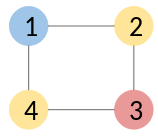
\includegraphics[height=2.1cm,width=2.3cm]{images/graphs/exampleGraph2.png}
  \caption{graph G$_{p}$}
  \label{fig:exampleGraph2}
\end{minipage}%
\begin{minipage}[t]{.6\textwidth}
  \centering
  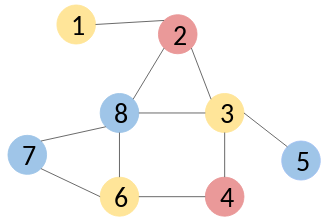
\includegraphics[height=3.4cm,width=5cm]{images/graphs/exampleGraph.png}
  \caption{graph G$_{t}$}
  \label{fig:exampleGraph}
\end{minipage}%
\caption{Instance of subgraph isomorphism problem (SIP)}
\label{fig:SIP}
\end{figure}

%% induced : if edge in p, then edge in t, but if edge not in p then edge not in t
%% non-induced: if edge in p, then edge in t
\subsection{The Subgraph Isomorphism Problem}

A graph G$^{\prime}$(V$_{G^{\prime}}$, E$_{G^{\prime}}$, L$_{G^{\prime}}$) is a \textit{subgraph} of G if and only if the vertices, edges and labels of G$^{\prime}$ are subsets of the vertices, edges and labels of G, that is V$_{G^{\prime}}$ $\subseteq$ V$_{G}$ and E$_{G^{\prime}}$ $\subseteq$ E$_{G}$ and L$_{G^{\prime}}$ $\subseteq$ L$_{G}$.

The \textit{\gls{sip}} between a graph G$_{p}$(V$_{p}$, E$_{p}$, L$_{p}$), called pattern and graph G$_{t}$(V$_{t}$, E$_{t}$, L$_{t}$), called target, is to find a function $f$ that maps a different vertex of the target to every vertex in the pattern such that for every v $\in$ V$_{p}$, v = $f$(v) and L$_{p}$(v) = L$_{t}$($f$(v)), where $f$(v) $\in$ V$_{t}$; and for all pairs of vertices u,v $\in$ V$_{p}$, (u, v) $\in$ E$_{p}$ $\Leftrightarrow$ (f(u), f(v)) $\in$ E$_{t}$. In other words, a valid mapping of G$_{p}$ to a subgraph in G$_{t}$ preserves the labeling and the set of neighbours (and therefore the degree) of each vertex in G$_{p}$. If $f$ exists, we say that the \gls{sip} instance is \textit{\gls{sat}}, i.e. it has at least one solution, otherwise it is \textit{\gls{unsat}}, i.e. there are no solutions.

\gls{sip} can be \textit{induced} or \textit{non-induced}. The induced version also requires that if \textit{v} $\nsim_{G_{p}}$ \textit{w}, then \textit{$f$(v)} $\nsim_{G_{t}}$ \textit{$f$(w)}. In this work, we discuss only the non-induced \gls{sip} that does not have this requirement.

When a valid matching function $f$ exists that maps vertex \textit{v} $\in$ G$_{p}$ to vertex \textit{w} $\in$ G$_{t}$, we write \textit{v} $\rightarrow_{f}$ \textit{w}. 

\begin{example}
Lest us consider the \gls{sip} instance (G$_{p}$, G$_{t}$) displayed in Figure \ref{fig:SIP}. This instance is \gls{sat}, because a function $f$ exists that produces a valid mapping of each vertex $\in$ G$_{p}$ to a vertex $\in$ G$_{t}$. For instance, 1 $\rightarrow_{f}$ 8, 2 $\rightarrow_{f}$ 3, 3 $\rightarrow_{f}$ 4 and 4 $\rightarrow_{f}$ 6. However, if 4 $\in$ G$_{t}$ was labeled in Y, then the \gls{sip} instance (G$_{p}$, G$_{t}$) would be \gls{unsat}, because no valid mapping that associates each vertex in G$_{p}$ to different vertex in G$_{t}$ would exist.
\end{example}

% \gls{sip} is NP-complete, however there exist a number of different approaches to solve it, some of which are ... 
There are various existing algorithms for the subgraph isomorphism problem \cite{vf2,Solnon:2010,CP2015,Larrosa:2002,Bonnici:2013,Zampelli:2010}. More thorough analysis of the problem and discussion on existing work is presented in Section \ref{sec:sipalgos}.

\subsection{The Filter-Verification Paradigm}
A set of target graphs is called a \textit{database} and it is denoted by \textit{T}. A set of pattern graphs, also known as \textit{query set} or \textit{queries}, is denoted by \textit{P}. A \textit{dataset D} is composed of \textit{T} and \textit{P}. 

\textit{Subgraph query processing} is, when given a set of query graphs, for each query return all graphs from the database that contain the query. These graphs form the \textit{answer set} $\fancyA_{q}$ of the corresponding query \textit{q}. A way to perform subgraph query processing is to run a \gls{sip} algorithm for every instance (G$_{p}$, G$_{t}$) $\in$ P$\times$T, where G$_{p}$ $\in$ P and G$_{t}$ $\in$ T.

\begin{example}
Let us consider again Figure \ref{fig:SIP} and assume that it represents a dataset \textit{T}, where Figure \ref{fig:exampleGraph2} is the query set, which contains only G$_{p}$, and Figure \ref{fig:exampleGraph} represents the graph database, which contains G$_{t}$. Then, subgraph query processing would solve the \gls{sip} (G$_{p}$, G$_{t}$), because \textit{P}$\times$\textit{T} = (G$_{p}$, G$_{t}$), returning $\fancyA_{G_{p}}$ = \{G$_{t}$\}, as \gls{sip} (G$_{p}$, G$_{t}$) is \gls{sat}.
\end{example}

%% todo: cite the np-complete part
Another way of processing queries is the \textit{filter-verification framework}, which consists of two steps. The \textit{filter} step tries to prune targets that can not be matched to a given query. The set of targets left after this step formes the set of \textit{candidates}, denoted as $\fancyC_{p}$, where $\fancyC_{p}$ $\subseteq$ T. The following \textit{verification} step then performs \gls{sip} for every pair (G$_{p}$,$\fancyC_{G_{p}}$) $\in$ P $\times$ $\fancyC_p$. The usage of the filter-verification paradigm is motivated by the fact that subgraph isomorphism is NP-complete and reducing the number of \gls{sip} calls by discarding targets that are \gls{unsat} for a given pattern during the filtering step and performing \gls{sip} using the limited set of candidates would yield to significant performance improvement \cite{ctindex,foteini}.

There are number of subgraph query processing algorithms based on the filter-verification framework \cite{ctindex,gcode,graphgrepsx,tree+delta>=graph,GRAPES}. This approach is discussed in more detail in Chapter \ref{ch:existingWork}, where more definitions and annotations are introduced in Section \ref{sec:filterVerificationParadigm} followed by analysis of related work in Section \ref{sec:ctindex} and Section \ref{sec:otherindexes}.

% how do we build the database index?
% using a pre-built index of the database, denoted as $\fancyI_{T}$

% what is a candidate set?
% graph index, features, ...
% what is false-positive? what is false-negative, why it can't exist?
\section{Report Organization}

%%%%%%%%%%%%%%%%%%%%%%%%% CHAPTER 2 %%%%%%%%%%%%%%%%%%%%%%%%%%%%
\chapter{Review of existing work}
\label{ch:existingWork}
\section{The nature of the problem}

%%%% datasets
\section{Datasets}
\label{sec:datasets}

    In this work we consider undirected graphs. We assume that, in each graph, each vertex has a unique identifier and in the graph database each graph has a unique identifier. 

This section gives more information about the datasets that were used to check the correctness and performance of the algorithm implementations. All graphs in these datasets are undirected.\par
\textbf{AIDS} is the standard database of the Antiviral Screen dataset of the National Cancer Insitute \cite{datasets}. The database has 40 000 molecules, represented as graphs. 

\begin{table}
\centering
\renewcommand{\arraystretch}{1.4}% Spread rows out...
\begin{tabular}{ >{\bfseries}m{1.5in} >{\centering}m{0.5in} >{\centering}m{0.5in} >{\centering}m{0.5in} >{\centering\arraybackslash}m{0.5in}  } 
\toprule
   						   & aids   & pcms  & pdbs  & ppigo \\
\midrule
 \# graphs 				   & 40 000 & 200	& 600   & 50 \\
 \# disconnected graphs$*$ & 3 157  &		&		&  \\ 
 \# distinct node labels   & 62	    &		& 		&  \\ 
 \# distinct edge labels   & 0 		& 0		& 0		& 0 \\ 
 avg \# edges			   & 46.95  & 		&		&  \\ 
 median \# edges		   & 	    &		&		&  \\ 
 avg \# nodes			   & 45		&		&		&  \\ 
 avg degree				   & 2.09	&		&		&  \\ 
 median \# nodes	       &		&		&		&  \\ 
 avg \# node labels		   & 4.4	&		&		&  \\ 
 median \# node labels     &		&		&		&  \\
 \bottomrule
\end{tabular}
\caption{Statistics about the datasets}
\label{table:datasets}
\end{table}    


\begin{table}
\centering
\renewcommand{\arraystretch}{1.3}% Spread rows out...
\begin{tabular}{ |>{\bfseries}m{0.5in} |>{\centering}m{0.8in}| >{\centering}m{0.8in}| >{\centering}m{0.8in}| >{\centering}m{0.8in}| >{\centering\arraybackslash}m{0.8in}|} 
\hline
 dataset & number of graphs & unique vertex labels & average node degree  & min node degree & max node degree\\
\hline
AIDS & 40 000 & 62 & 2.09 & ne znam & ne znam \\
\hline
PCMS & 200 & 21 & 23.01 & ne znam & ne znam \\
\hline
PDBS & 600 & 10 & 2.06 & ne znam & ne znam \\
\hline
PPIGO & 20 & 46 & 10.87 & ne znam & ne znam\\
\hline
\end{tabular}
\caption{Characteristics of the datasets}
\label{table:datasets}
\end{table}    


\small{$*$ A graph G is said to be disconnected if there exist two nodes in G such that no path in G has those nodes as endpoints.}

    The input we are working with is a file with the following format:\newline
    
    - put a table with the datasets and more information about them \\ 
    - average, median, etc. \\
    - say we work only with undirected graphs \\
    - say whether we consider induced/ non-induced subgraph isomorphism \\

\subsection{Subgraph Isomorphism Answers}
Each query in each query set matches at least one graph in the target set. Some queries match more than one graph. Below we give some statistics on number of target graphs matched.

\begin{table}
\centering
        \renewcommand{\arraystretch}{1.5}% Spread rows out...
        \begin{tabular}{l|r|r|r|r|r|r|r|r|}
            \cline{2-9}
            &
             \multicolumn{2}{c}{\textbf{AIDS}} & 
             \multicolumn{2}{|c}{\textbf{PCMS}} & 
             \multicolumn{2}{|c|}{\textbf{PDBS}} & 
             \multicolumn{2}{c|}{\textbf{PPIGO}} \\
            \cline{2-9}
              & number  & percent & number & percent & number & percent & number & percent \\
              \hline
            \multicolumn{1}{|l|}{\textbf{all SIP calls}}  &240,000   &100 &1,800 &100 &3,600 &100 &100 &100 \\
            \multicolumn{1}{|l|}{\textbf{SAT SIP calls}}  &20,816 &8.67 &592 &32.8 &2,780 &77.22 &61 &61 \\
            \multicolumn{1}{|l|}{\textbf{UNSAT SIP calls}} &219,184 &91.33 &1,208 &67.2 &820 &22.78 &39 &39 \\
            \hline
        \end{tabular}
        \caption{Number of SIP instances for each dataset and how many of them are SAT and UNSAT}
        \label{table:dataSAT}
    \end{table}


\section{Filtering-verification paradigm}
\label{sec:filterVerificationParadigm}
- smaller $C$, less time spent on subgraph isomorphism check, but more tie spent on indexing process

	\section{Motivation for usage}
    \section{What makes an index "good"}
	\section{Common techniques}
    	\subsection{Graph-mining}
    	\subsection{Non-graph-mining}
        \label{subsec:non-data-mining}
    \section{Methods with respect to choice of indexing unit}
        \subsection{Path-based indexing approach}
        Follows the general idea: enumerate all the existing paths in a database up to \textit{maxLen} length and index them, where a path is a vertex-edgeProperty-vetex sequence. *example*
        In order to create an index of a graph \textit{g}, this approach breaks \textit{g} into paths and in this way, the structural information of \textit{g} could be lost. This leads to more false-positive answers returned after the   
        Advantages:
        \begin{enumerate}
            \item Paths are easier to manipulate than trees and graphs.
            \item The index space is predefined: all the paths up to             \textit{maxLen} length are selected.
        \end{enumerate}
        
        Disadvantages:
        \begin{enumerate}
            \item Path is too simple: structural information is lost
            \item There are too many paths: the set of paths in a graph database usually is huge.
        \end{enumerate}
        \subsection{Tree-based indexing approach}
        
\subsection{CT-Index}
\label{sec:ctindex}
%%%%%%%%%%%%%%%%%%%%%%%%%%%%%%%%%%%%%%%%%%%%%%%%%%%%%%%%%%%%%%%%%%%%%%%%%%%%%
%%%                               CT-Index                               %%%%
%%%%%%%%%%%%%%%%%%%%%%%%%%%%%%%%%%%%%%%%%%%%%%%%%%%%%%%%%%%%%%%%%%%%%%%%%%%%%
% TODO: move this to a background information section
%%% TODO: give a definition of a path in a graph : A path in a graph is a sequence of distinct vertices, such that each successive pair of vertices are adjacent; we also allow a path from a vertex to itself, in which case the first and last vertices in the sequence are the same (and there is a cycle).
% TODO: prove that from paths we can safely discard graphs as not subgraph isomorphic if they don't have the same paths.

%
%
% NOTE 1 FROM PATRICK
% You need to be consistent. There is confusion between vertices and nodes. Please resolve this
% What I have done (and you might state) is that we assume nodes are in trees constructed from a pattern or target
% graph composed of vertices and that you do this to distinguish between the two
%
CT-Index \cite{ctindex} is divided into two main parts, filtering and verification, both described below. Also presented is a complexity analysis of the algorithms used by CT-Index and an empirical study of its performance (using an open-source Java implementation).
CT-Index supports data sets with edge and vertex labels and also wild card patterns. Although not explicitly stated in \cite{ctindex}, CT-Index addresses the non-induced subgraph isomorphism problem  ( definition \ref{def:subgraphIsomorphism}).

\subsubsection{Filtering}
During the filtering step, the features of all graphs in the target data set are extracted and saved to a file, i.e. the target index. The index is then used to filter out target graphs that cannot contain the pattern.  Features are specific subgraphs used to classify graphs, and are stored as hash-key fingerprints. Features may be paths, subtrees or cycles of bounded length. Since vertices and edges may contain labels, these features can be viewed as strings from a specified alphabet (where the alphabet is the labels). In \cite{ctindex} it is stated that the reason for using trees and cycles (as well as paths) is that ``trees capture additional structural information" and cycles ``represent the distinct characteristic of graphs ... often neglected when using only trees as features".

%
% NOTE 2 FROM PATRICK
% Note simple way to use maths
%
Although the time complexity of computing all features of a graph is not reported, it can be derived as follows. To extract a subtree of graph $G$ with $maxT$ number of edges, one starts with initially empty tree and repeatedly adds edges to extend the vertices that are in the current tree via the recursive function $ExtendTree$. We write $F$ for the set of every edge $(u,v)$ in $G$ and vertices $u$ and $v$ that belong to $G$, such that one vertex (say, $u$) is part of the current tree and the other (say, $v$) is not. If we have $n$ number of vertices in the current tree, each with degree $d$, then the size of $F$ is at most $n(d-1)$. $ExtendTree$ extends the current tree with a specified edge as parameter, generates $F$ and makes a recursive call for every edge in $F$, until the tree reaches size $maxT$.
%%% todo for the big O
In the start of the tree extraction when adding the first edge to the empty tree, the vertices on both ends of the edge are also added as part of the tree. Therefore, the size of $F$ initially is $2.(d-1)$. After every recursive call, one more vertex is added to the tree, which introduces $(d-1)$ new edges. That makes a total of $maxT+1$ vertices that will be added to the tree and $(maxT+1).(d-1)$ visited edges. Consequently, the complexity of extracting tree features is $\mathcal{O}(|E|.(maxT+1).(d-1))$. From this formula one can see that the number of edges in the graph has significant impact on the performance of the algorithm. When increasing the graph density, the algorithm will have slower performance, caused by the degree of each vertex and the total number of edges, which both will increase.

CT-Index computes a unique representation of each distinct feature, its \emph{canonical form}, and stores its string encoding in the index file. Thus, the equality of two features can be checked by testing the equality of their canonical forms. The canonical label of a tree feature is computed as follows: (1) find the root node $r$ of the tree, (2) impose a unique ordering of the children of each node. Step (1) is computed by repeatedly removing all leaf nodes of a tree until a single node or two adjacent nodes remain. In the first case, root $r$ is the last node left. In the second case the edge connecting the two remaining nodes are removed to obtain two trees, each with one of the remaining nodes as a root. 
Step (2) is based on the ordering of edge and vertex labels. For each node $p$ that is a parent of nodes $u$ and $v$, deciding whether $u$ is before $v$ depends first on the labels of the edges $(p,u)$ and $(p,v)$, then on the labels of $u$ and $v$ and finally on the subtrees of $u$ and $v$. A bottom-up approach is used (i.e. start with the nodes in the lowest level and move up towards the root) to compute this.

%%%% complexity of canonical label algorithm %%%%
Although not stated in \cite{ctindex} the complexity of their canonical labeling can be derived as follows. Step (1) is $\mathcal{O}(n)$, where $n$ is the number of nodes in the tree, as one needs to visit each node before removing it. The complexity of step (2) is as follows. We write $|p|$ for the number of interior nodes in the trees, which is equal to $n$ minus the number of leaf nodes. Step (2) visits a node, then visits its parent, and for every child of the parent node checks whether it should be first or second in the canonical label, using the vertex and edge labels conditions described above. This is repeated for every node in the tree up to the root. Therefore, the complexity of step (2) is $\mathcal{O}(|p|.|c|^{2})$, where $|c|$ denotes the number of children of a parent.

%%% 
In \cite{ctindex} it is claimed that step (2) is not linear time but is tolerable because ``... the trees occurring as features usually are small and vertex and edge labels are diverse and hence the order can be solved quickly". Therefore, we might assume that CT-Index is designed to support only specific types of data sets and that there exists data sets with less label diversity and with big trees as features that would result in poor performance. More specifically, as $maxT$ increases, or average degree increases, so too does the cost of step (2), and performance suffers (and we conduct experiments to test this hypothesis in section \ref{sec:ct-index-performance}).


\subsubsection{Fingerprints}
%%%% hash-key fingerprints %%%%
CT-Index uses a storage technique called \emph{hash-key fingerprint} to capture the features in the graph. A separate fingerprint is computed from the canonical labels for each graph in the database. A fingerprint is an array of bits and denotes whether a particular feature occurs in the graph or not. As there is no predefined set of possible features for each graph, reserving one bit for each feature in the feature set is considered infeasible\footnote{However, due to the restricted alphabet of labels it may be possible to enumerate all possible features thus avoiding some of the pitfalls of hashing, such as collisions and sensitivity to hash table size.}. A hash function maps extracted features to bit positions.
CT-Index is not the first indexing algorithm to employ fingerprints as a storage technique. The chemical information system called Thor and developed by Daylight \cite{fingerprints} is an example of an information processing system that uses bit arrays to store the features of the graphs.

%%%
Depending on the quality of the hash function, the size of the bitset and the size of the fingerprint, collisions may occur, i.e. different features may map to the same bitset position, introducing false-positives. The \cite{ctindex} paper briefly discussed some optimization techniques that could be used to minimize the influence of collisions, but it is unclear whether CT-Index employs them. 
It is stated that ``... the loss of information caused by the use of hash-key fingerprints seems to be justifiable by the compact nature and convenient processing of bit arrays as long as the amount of false positives does not increase significantly due to collisions".

Collisions can occur also if the size of the fingerprint is too small for the particular data, i.e. there is bigger number of features than the number of spaces in the array to store them. On the other hand, making the fingerprint size too big introduces additional overhead by requiring more memory storage space that is not used. The paper does not specify the hash function used or how to decide on the size of bitsets (feature hash tables). 

%%%% advantages %%%%
The main advantage of hashing the features and storing them in arrays is that this makes certain operations much cheaper. For example, checking whether a pattern fingerprint is included in a target fingerprint involves inexpensive bit operations. In particular, one only needs to compute a bitwise AND-operation with the two fingerprints to determine if features in the pattern exist within the target. If this test returns false then the target cannot be a candidate for that pattern. However, if it returns true then the target \emph{may} be a candidate and subgraph isomorphism must be verified.
%%%%%%%%%%%%%%%%%%%%%%%%%%%%%%%%% 
\subsubsection{Verification}
The verification step checks all candidates computed in the filtering step via a subgraph isomorphism test. A backtracking algorithm \cite{backtracking-algorithms}, similar to VF2 \cite{vf2} with additional heuristics, is used.  This test is theoretically NP-Complete, and is avoided as far as possible via the filtering process. CT-Index is not alone in using (essentially) the VF2 algorithm.
For example it is used in GraphGrepSX \cite{graphgrepsx}, gCode \cite{gcode} and Tree+$\Delta$ \cite{tree+delta>=graph}. Most papers claim that VF2 is ``state of the art".  However, this is not the case (\cite{Solnon:2010,Larrosa:2002,Bonnici:2013,Zampelli:2010,CP2015}.
VF2 has been shown to perform erratically and poorly \cite{CP2015}. Therefore we might summarise CT-Index architecture as using a potentially expensive indexing and filtering stage in order to minimise the computational cost of using an outdated subgraph isomorphism problem (SIP) algorithm.

%%%%%%%%%%%%%%%%%%%%%%%%%%%%%%%%%
\subsubsection{Performance}
\label{sec:ct-index-performance}
%%%% foteini's paper %%%%
%%%% TODO rewrite that part %%%$
This section describes the performance 
We searched for more information in alternative sources. In \cite{foteini} the authors compare several well-established indexing techniques, including CT-Index and try to draw conclusions on their performance depending on a set of key-factor parameters. The authors use the four datasets described in section \ref{sec:datasets} as well as a synthetically generated database of targets and queries to conduct their experiments. These are some of the conclusions made after the experiments:
\begin{itemize}
%\item Datasets with increased number of distinct labels are easier and faster to index and compute subgraph isomorphism answers.\newline
%The reason for this result is straightforward, as the more distinct labels a graph has, the easier it is to discard nodes as possible matches to a pattern node, taking only the labels of nodes and edges into account.
\item The size of the query affects the performance of the indexing method\newline
This conclusion is also very easy to obtain. As the size of the pattern becomes larger, there are more nodes that have to be matched to a target node. Suppose that we have a pattern graph $p$ with $|p|$ number of nodes and a target graph $t$ with $|t|$ number of nodes that is a candidate for subgraph isomorphism. Assume that all techniques to discard $t$ before the search have failed, i.e. $|t|$ $\geq$ to $|p|$, etc. Then, for each node in $p$, the ct-index algorithm tries to map to a node in $t$ and continues until either it either fails or succeeds. In the first case, the algorithm backtracks and tries to map an alternative node from $t$ and in the second case, the algorithm terminates, as a valid map of all pattern nodes to some of the target nodes is found. One can easily notice that the bigger the size of $|p|$, the more checks the subgraph isomorphism algorithm will do. The same conclusion could be reached for $|t|$. When there are more nodes in $t$, more different ways exist for matching a node in $p$ to a node in $t$.
\item CT-Index has relatively small index size, compared to other indexing techniques.\newline
Again, this result could be obtained even without running any experiments. As the CT-Index uses bitset arrays to store the features, it straightforward to reach to the conclusion that CT-Index always has smaller index size, compared to other techniques that do not compress the features, but directly store them in the index file.\par
\end{itemize}
%%%
The results from \cite{foteini} have a major limitation: for each indexing methods, the authors use the "default" input parameter values, given by the original authors of each of the indexing methods. They never experiment with alternative values. It is not clear why the corresponding input values are fair and the best ones to use and why the authors do not consider the possibility of obtaining completely different results if they changed the input parameters values. Also, the authors never say whether they have checked how they verified that the indexing methods compared in the paper give correct results.\par
%%%% our evaluation %%%%
We conducted a separate evaluation using the implementation and the datasets descried in section \ref{sec:datasets}. Table \ref{table:runningTime} shows the running time of CT-Index: time to build the index, time to compute answers out of the set of candidates and the total running time depending on the values of the parameters specified for the AIDS dataset, namely the size of the fingerprint, the maximum bound for path, subtree and cycle size; and the number of candidates for after indexing and filtering for the corresponding query number. Table \ref{table:answers} shows the actual number of targets that contain the particular query as subgraph. This can be used to check the ratio of false-positives against real results for each query for each of the different input parameter values. We write -1 as the value of maximum path, cycle or subtree length whenever we do not want to use the corresponding structure as feature. We recorded the running time of both indexing and querying, as well as the number of candidates, because in real applications, the index is computed once and then reused multiple times, until the target dataset is changed. This means that for applications that require frequent changes to the database it is desirable to compute the index as fast as possible, whereas for datasets that are rarely changed, the time to compute the index is not that important and one may focus on increasing the quality of the index (i.e. it leads to smaller number of candidates).\par
To verify the correctness of the results obtained by CT-Index and later on be able to use the implementation as a benchmark, we did the following activities. As we did not have set of answers for each query, we first computed the answers for each query, varying the input parameters values. We verified that all results are the same by executing a script that checks whether every set of answers a query is the same as every set of answers obtained for the same query, but with different parameter values. Finally, we used a subgraph isomorphism solver program that does not employ indexing to compute the answers for each query and we compared these answers with the CT-Index answers to conclude that they are the same and CT-Index is correct at least for the corresponding input parameter values.\par
%%% 
%%%% big table with ct-index running times and results on the AIDS dataset %%
\newcommand\TstrutT{\rule{0pt}{2.6ex}}         % = `top' strut
\newcommand\Bstrut{\rule[-1ex]{0pt}{0pt}} 
\begin{table}[H]
\caption{CT-Index: Running time and results}
\label{table:runningTime}
\begin{center}
\begin{tabular}{ |c|p{25mm}|c|c|c|p{18mm}|}\hline
 & fingerprint size \newline max path len\newline max subtree len \newline max cycle len & index build T[sec]& query T[sec]& total T [sec] & \textbf{query\#} \#candidates\TstrutT\Bstrut\\
 \hline
1& 4096 -1 \,5 \,5  & 82.376 & 5.896 & 88.272 & \textbf{0} 11 160 \newline \textbf{1} 13 577 \newline \textbf{2} 975 \newline \textbf{3} 2 950 \newline \textbf{4} 2 575 \newline \textbf{5} 6 \TstrutT\Bstrut\\ 
 \hline
2 & 4096 \,5 \,5 \,\,5 & 108.465  & 5.948 & 114.413 & \textbf{0} 11 168 \newline \textbf{1} 13 589 \newline \textbf{2} 1058 \newline \textbf{3} 2 949 \newline \textbf{4} 2 576 \newline \textbf{5} 6 \TstrutT\Bstrut \\ 
 \hline
3 & 4096 \,5 -1 -1 & 37.621  & 7.929 & 45.550 & \textbf{0} 31 083 \newline \textbf{1} 36 458 \newline \textbf{2} 4 285 \newline \textbf{3} 7 261 \newline \textbf{4} 13 316 \newline \textbf{5} 252 \TstrutT\Bstrut \\ 
 \hline 
4 & 4096 \,5 \,\,1 \,\,1 & 41.482  & 7.96 & 49.442 & \textbf{0} 31 083 \newline \textbf{1} 36 458 \newline \textbf{2} 4 285 \newline \textbf{3} 7 261 \newline \textbf{4} 13 316 \newline \textbf{5} 252 \TstrutT\Bstrut\\ 
 \hline
5 & 2048 \,5 \,\,1 \,\,1 & 41.269  & 13.295 & 54.564 & \textbf{0} 31 085 \newline \textbf{1} 36 458 \newline \textbf{2} 4 293 \newline \textbf{3} 8 539 \newline \textbf{4} 13 319 \newline \textbf{5} 252 \TstrutT\Bstrut\\ 
 \hline
6 &  2048 \,-1 \,\,5 \,\,5 & 87.959  & 8.22 & 96.179 & \textbf{0} 11 540 \newline \textbf{1} 13 582 \newline \textbf{2} 987 \newline \textbf{3} 2 983 \newline \textbf{4} 2 660 \newline \textbf{5} 9 \TstrutT\Bstrut\\ 
 \hline
\end{tabular}
\end{center}
\end{table}
%%%
%%%% Analysis of the big table %%%%
Looking at rows 1 and 2, we can conclude that extracting paths as features as well as subtrees and cycles leads to significantly slower index built time and slightly worse filtering power. Comparing row 1 and row 3, one can see that extracting only paths takes significantly lower amount of time, compared to using only trees as features. However, it leads to worse filtering power. The results from rows 1, 2 and 3 support the claim that trees are much more descriptive features than paths. Also, they show that using paths, subtrees and cycles all together as features leads to slower running time.\par
%%%
As it can be seen that the rows with the smallest number of candidates are the ones that store trees in the index file (rows 1, 2 and 6), these are also the instances with the slowest index built time. The reason could be that trees are more complex than paths and require more time to be extracted and transformed to unique string representations. As explained in the previous section, the authors use algorithm that computes the canonical form the the features of high complexity. Maybe if the authors used more optimal algorithm, it would lead to faster running time.\par
%%%
As it can be seen in column 5 of table \ref{table:runningTime}, the total running time of CT-Index varies from 49 seconds to 114 seconds depending on the specified input parameters. If we look at rows 4 and 5, the only difference of the input parameter values is the fingerprint size. As it can be seen from the table, the time difference to build the index in 4 and 5 is only around 200 miliseconds. However, the time taken to compute the answers from the set of candidates is more than 6 seconds slower in row 5 compared to row 4, although the number of candidates for the two rows are almost the same for every query except query 3. Similar difference can be observed when comparing row 1 with row 6. The reason for these results could be that fingerprint of size 2048 is too small for the particular dataset and this leads to more collisions.\par
%%%
To conclude, in CT-Index, when using only paths as features leads to smaller running time for building index, however it significantly bigger number of candidates and therefore bigger amount of time to find all targets containing the query from the set of candidates. Using trees as features results to an index with much better filtering power, but slower to compute. Hashing features constructed from paths and trees does not give any benefit, moreover, it it slower and results to slightly bigger number of candidate graphs.\par

%%%% TODO write about the experiments with other data sets
%When running the implementation of \cite{ctindex}, we observed that the algorithm never terminated for some instances of pdbs and ppigo. A similar question arises here: it this because the indexing technique is insufficient to eliminate incompatible targets 
% TODO: write the answer of these questions:
% is it because of SIP of ct-index being really bad?
% is it the case that both SIP of ct-index is really bad and the indexing pat also takes a lot of time and is useless? Need to do ct-index data analyzing to be able to answer these questions.
%%% TODO add some plots 
\subsection{gIndex, gCoding .... mention them}
\label{sec:otherindexes}
\section{Subgraph Isomorphism Algorithms}
\label{sec:sipalgos}
\subsection{Partick and Ciaran's paper}
\label{sec:sippatrick}
\subsection{Christine's paper}
\label{sec:sipchristine}

\chapter{Path-based query processing algorithms based on filtering-verification }

The order of a graph is the cardinality of its
vertex set. We write V(G) for the vertex set of a graph G.

%A non-induced subgraph isomorphism from a graph P (called the pattern) to a graph T (called the target) is an injective mapping from V(P)to V(T) which preserves adjacency— that is, for every adjacent v and w in V(P), the vertices i(v) and i(w) are adjacent in T. An induced subgraph isomorphism additionally preserves non-adjacency—that is, if v and w are not adjacent in P, then i(v) and i(w) must not be adjacent in T. We use the notation i : P  T for a non-induced isomorphism, and i : P ,\→ T for an induced isomorphism.



%%%%%%%%%%%%%%%%%%%%%%%%%%%%%%%%% Benchmarks %%%%%%%%%%%%%%%%%%%%%%%%%%%%%%%%
\section{Benchmarks} %% not sure this is the best name for this 
This section includes more information about the already existing indexing algorithm implementations that were used as a standard point of reference against our graph indexing implementations. 
%%%%%%%%%%%%%%%%%%%%%%%%%%%%%%%%%





%%%%%%%%%%%%%%%%%%%%%%%%%%%%%% Index algorithms %%%%%%%%%%%%%%%%%%%%%%%%%%%%%
%%% todo move this to where I explain the filter-verification paradigm
\section{Index algorithms}

    All algorithms described in this section generate the candidate set of graphs in the following steps:
    
    \begin{enumerate}
        \label{indexSteps}
        \item Compute the index of all graphs in T;
        \item Compute the index of all patterns in P;
        \item Using the target and pattern indexes computed in the previous two steps, extract all graphs in T that contain all features in the pattern index;
        \item All extracted graphs from step 3 form the candidate set C.
	\end{enumerate}
    
    In this work, we consider only induced subgraphs (definition \ref{def:induced-subgraph} in section \ref{subsec:definitions}) and the induced version of the subgraph isomorphism problem (definition \ref{def:inducedSubgraphIsomorphism} in section \ref{subsec:definitions})
    
    The correctness of the results is checked comparing the answers obtained from CT-Index. We implemented a class called $Verify.java$ that checks whether the resulting candidate set after each query execution contains the answers of subgraph isomorphism. $Verify.java$ was very useful for discovering a lot of bugs during the software development process.
    
%%%%%%%%%%%%%%%%%%%%%%%%%%%%%%%%%%%%%%%%%%%%%%%%%%%%%%%%%%%%%%%%%%%%%%%%%%%
%%%%%%------------------------- Path Index --------------------------%%%%%%
%%%%%%%%%%%%%%%%%%%%%%%%%%%%%%%%%%%%%%%%%%%%%%%%%%%%%%%%%%%%%%%%%%%%%%%%%%%
\section{Path Index}
\label{path-index}
This section gives an overview of the first indexing technique that was designed and implemented. In following subsections we describe the main idea of the algorithm ans the implementation. The performance results that were obtained after running various types of queries on targets of varying size are described along with a summary of the advantages and limitations of the algorithm.\par
%%%%%%%%%%%%%%%%%%%%%%%%%%%%%%%%%%%%%%%%%%%%%%%%%%%%%%%%%%%%%%%%%%%%%%%%%%%
\subsection{The idea}
\label{path-index-idea}
    The algorithm uses an exhaustive path-enumeration approach to build its index. This technique is employed by various algorithms like CT-Index \cite{ctindex}, gCode \cite{gcode} and GraphGrepSX \cite{graphgrepsx}. The main idea behind \textit{exhaustive path-enumeration} is to enumerate all existing paths in a database up to $maxL$ length and index them, where a path is a sequence of vertexes such that each vertex is connected with an edge with the previous and the next vertex in the sequence.\par
%%%%%%%%%%%%%%%%%%%%%%%%%%%%%%%%%%%%%%%%%%%%%%%%%%%%%%%%%%%%%%%%%%%%%%%%%%%
   Given a set of target graphs $T$ and a pattern graph $p$, $Path$-$index$ first computes the index of all graphs in $T$ by enumerating exhaustively all paths in every target up to a specified maximum path length $maxL$. The paths are then stored in a file, which is the target$'$s index. The same procedure using the same value of $maxL$ is followed to derive the pattern index. The two files are then used for finding the candidate set $C$ of all graphs in $T$ that have to be checked for subgraph isomorphism with $p$. Using the pattern index, we check which targets contain all paths in the pattern index and filter out all targets that do not have all paths that the pattern does. The rationale behind this filtering method is that if some features of graph $p$ do not exist in a graph $t$, $t$ cannot contain $p$. However, if $t$ contains all features of $p$, this does not meant that $p$ is subgraph of $t$: $t$ can be a \textit{false-positive} and a subgraph isomorphism test needs to be performed on $t$ and $p$ to identify whether $t$ is a \textit{false positive} or it indeed contains $p$. All targets in $T$ that have all paths, extracted from the pattern graph, form the candidate set $C$. All graphs in $C$ are then checked for subgraph isomorphism with $p$. \par
%%%%%%%%%%%%%%%%%%%%%%%%%%%%%%%%%%%%%%%%%%%%%%%%%%%%%%%%%%%%%%%%%%%%%%%%%%%
As mentioned before, each path is a sequence of vertices of maximum size $maxL$, such that each vertex is connected with an edge with the previous and the next node in the sequence. Each path, extracted from the graph, is stored in the index file in a string representation, derived from the label of each node in the sequence and the label of the edge (if existent) between the node and its neighbors. In this work, we refer to these path string representations as path-strings. To avoid redundancy index comprises of unique path-strings, computed from the paths taking the following points into consideration:
\begin{itemize}
\item Path $a$ is equivalent to its reverse variant $a$-$reversed$, because the graphs in the datasets are undirected, as mentioned above. There is no need to store both $a$ and $a$-$reversed$ in the index, as this would lead to redundancy.
\item Path $a$ is not equivalent to a path $a$-$sorted$, where $a$-$sorted$ is the sorted variant of $a$ in lexicographical order (either increasing or decreasing). Sorting $a$ can change the places of some of the nodes that comprise the sequence, which means that some nodes may have different neighbors in the sorted path. This introduces new edges in $a$-$sorted$ that may not exist in $a$ or in the graph.
\end{itemize}
To avoid redundancy and make the index search faster, only one unique path-string is written to the file for each path and its equivalent path-string variants, derived using the properties mentioned above. We chose to add to the index the lexicographically smaller path-string between a path and its reverse. \par
%%%%%%%%%%%%%%%%%%%%%%%%%%%%%%%%%%%%%%%%%%%%%%%%%%%%%%%%%%%%%%%%%%%%%%%%%%%
   % example for both previous paragraphs%
Let the graph on figure \ref{B2Y5G} be a target graph in $T$ and the graph on figure \ref{CH4} be a pattern graph in $P$, where the number in red next to each node on the two figures denotes the id number of the corresponding vertex. Let $maxL$ be equal to 3. In order to check whether \ref{C5H12} is a candidate for subgraph isomorphism with \ref{CH4}, we first compute the indexes of \ref{C5H12} and \ref{CH4} for the specified maximum path length. The target index consists of the paths on figure \ref{C5H12-paths} and the pattern index contains the paths on figure \ref{CH4-paths}. There is a lexicographically smaller variant of the path-string \textrm{H-C-H}, namely \textrm{C-H-H}. However, no path in the the graph \ref{C5H12} can form such path-string and adding \textrm{C-H-H} to the index file could lead to wrong results.\par
%%%%%%%%%%%%%%%%%%%%%%%%%%%%%%%%%%%%%%%%%%%%%%%%%%%%%%%%%%%%%%%%%%%%%%%%%%%
\begin{figure}[H]
\centering
\begin{minipage}[t]{.5\textwidth}
  \centering
  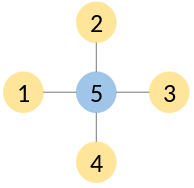
\includegraphics[height=3cm,width=3.3cm]{images/graphs/CH4.png}
  \caption{Pattern graph P}
  \label{CH4}
\end{minipage}%
\begin{minipage}[t]{.5\textwidth}
  \centering
  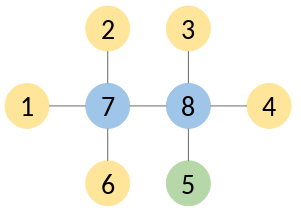
\includegraphics[height=3cm,width=4.2cm]{images/graphs/B2Y5G.png}
  \caption{Target Graph T}
  \label{B2Y5G}
\end{minipage}
\end{figure}
%%%%%%%%%%%%%%%%%%%%%%%%%%%%%%%%%%%%%%%%%%%%%%%%%%%%%%%%%%%%%%%%%%%%%%%%%%%
After candidate extraction, Path-Index returns target graph \ref{B2Y5G} as candidate for subgraph isomorphism with pattern graph \ref{CH4}, as all paths in \ref{CH4}, shown on figure \ref{CH4-paths} are contained in \ref{C5H12}, as it can be seen on figure \ref{C5H12-paths}.\par
%When the set of targets is the same for multiple patterns, the target index is still computed only once and reused. The 
%%%%%%%%%%%%%%%%%%%%%%%%%%%%%%%%%%%%%%%%%%%%%%%%%%%%%%%%%%%%%%%%%%%%%%%%%%%
\begin{figure}[H]
\centering
\begin{minipage}[t]{.5\textwidth}
  \centering
  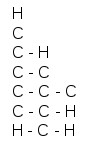
\includegraphics[height=3.3cm,width=2.3cm]{images/paths/C5H12.png}
  \caption{Target graph path enumeration}
  \label{C5H12-paths}
\end{minipage}%
\begin{minipage}[t]{.5\textwidth}
  \centering
  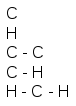
\includegraphics[height=2.4cm,width=2cm]{images/paths/CH4.png}
  \caption{Pattern graph path enumeration}
  \label{CH4-paths}
\end{minipage}
\caption{All paths up to maximum length 3}
\label{pathsEnumeration}
\end{figure}
%%%%%%%%%%%%%%%%%%%%%%%%%%%%%%%%%%%%%%%%%%%%%%%%%%%%%%%%%%%%%%%%%%%%%%%%%%%
\subsection{Implementation}
\label{path-index:implementation}
\subsubsection{Graph representation}
\label{path-index:graph-representation}
	Each graph is represented with a Java class \textrm{Graph} that has an integer id and a collection of node objects as fields, where the integer is a unique identifier. Each node object has an id, a label and a list of edge objects, where the node is a source node for each edge contained in the list. The length of the list of the edge object is equal to the degree of the node. Therefore, each edge object does not need to keep a record of the source node: it only has a label and a destination node as fields. As the graphs we are working with are not directed, two Edge objects are created to represent an edge. The first object has one of the nodes as destination node and then added in the list of edges of the other node: the source node. The second edge object will have the source node of the first edge object as destination node and included in the list of edges of the destination node of the first edge object, which will be its source node. The label of both edge objects will be the same.\par
%%%%%%%%%%%%%%%%%%%%%%%%%%%%%%%%%%%%%%%%%%%%%%%%%%%%%%%%%%%%%%%%%%%%%%%%%%%
\subsubsection{Path Extraction}
\label{path-index:path-extraction}
A class, called \textrm{PathExtractor}, contains all functionality for computing the paths and path-strings that are stored in the index. To compute the index of a given graph dataset, we use the functionality of \textrm{PathExtractor} to extract all paths of every graph in the dataset. The path extraction algorithm is recursive depth-first-search based and is called on every node of the graph. Algorithm 1 describes our approach. Before we call function \textrm{generatePath}, we initialize an empty stack that is used in the algorithm to store visited nodes. \textrm{Algorithm 1} generates all paths in the graph of size $maxL$ , where $maxL$ is the number of nodes in a path, using two functions: \textrm{generatePath} and \textrm{generatePathInner}. The function \textrm{generatePath} in \textrm{Algorithm 1} takes a list of all nodes in the graph and path length $maxL$ as parameters and calls \textrm{generatePathInner} for every node in the list as starting node (line 4). The start node is also pushed on the stack (line 3), as it is part of the path that is to be generated. \par

%%% proper path extraction algorithm
\begin{algorithm}
\centering
\caption{Paths extraction}
\label{alg:generatePath}
\begin{algorithmic}[1]
\Procedure{generatePath }{nodes, l$_{max}$, s}
\For{node in nodes}
	\State s $\gets$ init \Comment{\textit{initialize the stack}}
	\State push node on top of s
	\State \Call{generatePathInner}{node, l$_{max}$, s}
\EndFor
\EndProcedure
\end{algorithmic}
\end{algorithm}
%%% end of algorithm

%%% generatepath inner algorithm
\begin{algorithm}
\centering
\caption{Paths extraction}
\label{alg:generatePathInner}
\begin{algorithmic}[1]
\Procedure{generatePathInner }{node, l$_{max}$, s}
\If{s $\leq$ l$_{max}$}
\State new path $\gets$ s \Comment{\textit{new path of size is found}}
\EndIf
\If{s == l$_{max}$}
\State s.pop()
\EndIf
\For{neighbour of node}
\If{neighbour not in s}
\State s.push(neighbour)
\State \Call{generatePathInner}{neighbour, l$_{max}$, s} \Comment{\textit{recursive call}}
\EndIf
\EndFor
\If{s is full} \Comment{\textit{all neighbours of node are on the stack}}
\State s.pop()
\EndIf
\EndProcedure
\end{algorithmic}
\end{algorithm}
%%% end of algorithm
%%% end of path extraction algorithm


%TODO explain lines 7 - 11 and check the correctness of line numbers
The recursive function \textrm{generatePathInner} generates all paths is length $maxL$, where the length of a path is equal to the number of all nodes that are part of it, from a start node $node$. First, the size of the stack is checked. If it is less or equal to $maxL$, the contents of the stack are copied and passed to a function \textrm{putToIndex} that computes the string representation of the extracted path and puts it to the index. If the stack is equal to $maxL$, the last element from the stack is popped out and the function exits. If the size of the stack is less than $maxL$, we traverse the neighborhood of $node$ in the for loop, starting at line 12. Every unvisited neighbor of $node$ is pushed on the stack and then a recursive call to \textrm{generatePathInner} is made with the same neighbor node as $node$(lines 13 and 14).\par
%%%%%%%%%%%%%%%%%%%%%%%%%%%%%%%%%%%%%%%%%%%%%%%%%%%%%%%%%%%%%%%%%%%%%%%%%%%
The stack used in \textrm{Algorithm 1} follows the principles of the stack datastructure. In this work, we use the Java implementation. The stack has two main functions: to keep track of the visited nodes in the current function call so that no node takes part in a path more than twice, i.e. there are no cycles; and it contains nodes that always form a valid path. The reason why this is the case is that every time a node is pushed on top of the stack, this node is one of the neighbors of the last node on the stack. The only place in generatePathInner function where new node is added in the stack is in line 14 and the node that is pushed on top of the stack belongs to the list of neighbors of $node$, which is always the previous node in the stack. Therefore, the sequence of all nodes on the stack forms a valid path, as every node is connected with an edge with its predecessor and successor in the sequence. The complexity of Algorithm 1 is explained in section \ref{path-index:complexity}.\par
%%%%%%%%%%%%%%%%%%%%%%%%%%%%%%%%%%%%%%%%%%%%%%%%%%%%%%%%%%%%%%%%%%%%%%%%%%%
The function \textrm{outputPath} is called by \textrm{generatePathInner} every time the stack reaches a size equal to $maxL$ (line 8, Algorithm 1). Algorithm 2 derives the lexicographically smallest string representation of a path, following the principles described in section \ref{path-index-idea}. The resulting path-string is added to the index, if it does not exist there (line 8, Algorithm 2). \par 
Algorithm 2 takes a sequence of nodes as a parameter, which are the contents of the stack when the stack size is $maxL$ (line 8, Algorithm 1). We derive the path-string of the sequence (line 2) that consists of the node label of every node in nodeSequence and the label of the edge it has with the previous node in the path. If the dataset does not have edge labels, a default character is used as label for every edge. In the previous examples, we use the character $"-"$ (figures \ref{C5H12-paths} and \ref{CH4-paths}). It is important to note that the node labels are ordered in exactly the same way as the nodes in the sequence, for example if a node A is on place \textit{i} in the sequence, the label of A will be at place \textit{i} in the string if the edge labels in the string are not counted (if they are counted, the label of A is at position \textit{i} x \textit{2}).\par
Next steps are to compute the reversed sequence of the path (line 3), its string representation (line 4) and check whether the reversed string is lexicographically smaller then the path-string (line 5). If yes, we assign the path-string to be equal to the reversed string (line 6) and add it to the index, if it is not present there yet (line 8). We do not sort the path-string lexicographically, due to the reasons explained in section \ref{path-index-idea}. The complexity of Algorithm 2 is explained in section \ref{path-index:complexity}.\par

%%% proper output path algorithm
%%% proper path extraction algorithm
\begin{algorithm}
\centering
\caption{Output path procedure}
\label{alg:generatePath}
\begin{algorithmic}[1]
\Procedure{getPath }{nseq}
\State pathStr $\gets$ nseq.toString() \Comment{\textit{returns a string of the labels of the nodes in nseq}}
\State rseq $\gets$ nseq.reverse() \Comment{\textit{reverse the order of nodes in nseq}}
\State pathStrRev $\gets$ rseq.toString() \Comment{\textit{returns a string of the labels of the nodes in rseq}}
\If {pathStrRev $<$ pathStr}
\State pathStr $\gets$ pathStrRev \Comment{\textit{put to index the lexicographically smaller string}}
\EndIf
\If {pathStr not in index}
\State add pathStr to index
\EndIf
\EndProcedure
\end{algorithmic}
\end{algorithm}
%%% end of algorithm


%TODO the bug I had initially, how the stack was fixed
% TODO reference Java stack below
% TODO explain about the current maximum path length
% TODO explain isVisited boolean field in the Node class
%Iteration is every new entering to the while loop when we have new start node and we have the stack cleaned up. --- write that properly
%%%%%%%%%%%%%%%%%%%%%%%%%%%%%%%%%%%%%%%%%%%%%%%%%%%%%%%%%%%%%%%%%%%%%%%%%%%
\subsubsection{Candidates extraction}
\label{path-index:candidates-extraction}
Candidates extraction is the part of the implementation where the set of candidates $C$ from the dataset with target graphs is constructed. Algorithm 3 describes our approach in more detail. Function \textrm{candidatesExtractor} takes the index of one graph from the target dataset and the index of the pattern (or one of the set of pattern graphs, if there are more than one pattern) as parameters (line 1). For every path-string in the pattern, we check whether it is contained in the target index (line 3). If yes, the algorithm continues, because the target might be a candidate (line 6). Otherwise, if the pattern path-string does not exist in the target index, the program returns false and terminates (line 4). The program goes to line 7 iff all path-strings in the pattern are contained in the target index.\par
The complexity of Algorithm 3 is explained in section \ref{path-index:complexity}. 

%%% proper candidates extraction algorithm
\begin{algorithm}
\centering
\caption{Candidates extraction}
\label{alg:candidatesExtraction}
\begin{algorithmic}[1]
\Procedure{candidatesExtractor }{$\fancyI_{G_{p}}$, $\fancyI_{G_{t}}$}
\For{path$_{p}$ in $\fancyI_{G_{p}}$}
\For{path$_{t}$ in $\fancyI_{G_{t}}$}
\If{no path$_{t}$ is equal to path$_{p}$} \Return false \Comment{\textit{path$_{p}$ is not in $\fancyI_{G_{t}}$, return false}}
\EndIf
\EndFor
\EndFor
\EndProcedure
\end{algorithmic}
\end{algorithm}
%%% end of algorithm

\subsection{Performance}
This section gives more details about the complexity of each of the algorithms in the implementation, explained in sections \ref{path-index:path-extraction} and \ref{path-index:candidates-extraction}, continued with statistics about the algorithm running time and performance after running it on various datasets. Following the results obtained, we make a conclusion about the observed performance of the algorithm and analyze its advantages and disadvantages.\par
%%%%%%%%%%%%%%%%%%%%%%%%%%%%%%%%%%%%%%%%%%%%%%%%%%%%%%%%%%%%%%%%%%%%%%%%%%%
\subsubsection{Complexity}
\label{path-index:complexity}
Algorithm 1 works like depth-first search, but the depth of the search has a maximum limit $maxL$. For each target graph, we conduct depth-first search of depth $maxL$. During the search, each neighbor of $maxL$ number of nodes is visited. The worst case complexity is when the target graph is a clique. If we assume that the number of nodes in the clique is n (equal to the number of edges), then the for loop on line 2 will be executed n times, each time calling \textrm{generatePathInner} function. This function will make recursive call for every unvisited neighbor of the current vertex, until the stack reaches size equal to $maxL$. As after every recursive call, the size of the stack is increased by 1 and the graph is a clique, the number of neighbors that will be visited during the next recursive call decreases by 1. The depth of the recursive calls is at most $maxL$ (the maximum size of the path we want  is $maxL$), therefore the function has worst case complexity \textbf{O((n - 1).(n - 2) ... (n - maxL - 1))}, which occurs when the graph is a clique. \par
%%%%%%%%%%%%%%%%%%%%%%%%%%%%%%%%%%%%%%%%%%%%%%%%%%%%%%%%%%%%%%%%%%%%%%%%%%%
 Algorithm 2 does not have any loops, but it calls the function \textrm{toString()}, which traverses the given path once to change each node with its label and an edge label to the next node in the sequence. The \textrm{toString()} method visits every node in the path, takes the label of the current node, and if the dataset has edge labels, finds the edge label of the edge between the current node and the next node, otherwise adds a default character after the node label. On line 7, there is a traversal through the current index of a graph. The complexity of Algorithm 2 is therefore \textbf{O(maxL + index size)}, where index size is the current size of the index for the current graph being indexed. The best case is when the index is empty: then traversing the index takes constant time and the complexity of the \textrm{toString()} method is \textbf{O(maxL)}.\par
%%%%%%%%%%%%%%%%%%%%%%%%%%%%%%%%%%%%%%%%%%%%%%%%%%%%%%%%%%%%%%%%%%%%%%%%%%%
Algorithm 3 visits every path stored in the pattern index and for each pattern path, it goes through the target index and checks whether it contains the same path. This procedure is done for every target graph in the dataset. If we assume that the number of paths in the pattern index is \textit{p}, the number of paths in the current target index is \textit{t} and the number of graphs in the target dataset is \textit{n}, the number complexity of the algorithm is \textbf{O(ptn)}.\par
%%%%%%%%%%%%%%%%%%%%%%%%%%%%%%%%%%%%%%%%%%%%%%%%%%%%%%%%%%%%%%%%%%%%%%%%%%%
\subsection{Experimental Results}
\label{path-index:experimental-results}
TODO


%%%%%%%%%%%%%%%%%%%%%%%%%%%%%%%%%%%%%%%%%%%%%%%%%%%%%%%%%%%%%%%%%%%%%%%%%%%
\subsection{Advantages and Limitations}
\label{path-index:advantages-limitations}
    TODO\\
    - structural information is lost, because path is too simple\\
	- it is computationally intense, i.e. very slow especially when computing paths of higher length; there are too many paths\\
    - very easy to implement\\
    - paths are easier to manipulate than trees and graphs --- why?\\
    - this indexing technique is good when we have graphs with large number of different labels on their nodes and low density of edges between the graphs' nodes\\
    - the index space is predefined: all the paths up to \texttt{maxLen} length are selected\\
%%%%%%%%%%%%%%%%%%%%%%%%%%%%%%%%%%%%%%%%%%%%%%%%%%%%%%%%%%%%%%%%%%%%%%%%%%%
%%%%---------------------- Path-Subtree Index -------------------------%%%%
%%%%%%%%%%%%%%%%%%%%%%%%%%%%%%%%%%%%%%%%%%%%%%%%%%%%%%%%%%%%%%%%%%%%%%%%%%%
\section{Path-Subtree Index}
\label{path-subtree-index}
  $Path$-$Subtree$ index is the second indexing technique that was designed, implemented and evaluated. In this section we explain its main idea, implementation and performance, observed after testing with various types of graph data sets. We write about the problems with the algorithm we discovered after the initial implementation and how we changed $Path$-$Subtree$ index to solve the issues encountered. Lastly, we draw conclusions about the advantages and limitations of this indexing technique.  
\subsection{Initial idea}
%%%%%%%%%%%%%%%%%%%%%%%%%%%%%%%%%%%%%%%%%%%%%%%%%%%%%%%%%%%%%%%%%%%%%%%%%%%%
As mentioned in section \ref{path-index:advantages-limitations}, $Path$ index can't extract most of the structural information present in the graphs. It is almost of no use for targets that have small number of different labels, like the AIDS data set for example. $Path$-$Subtree$ index addresses the problem of insufficient structural information extraction by introducing a novel representation of the paths that takes into account the neighborhood of each node. A new version of the label of each node that is present in the path is computed and stored in the index instead of the node$'$s original label. In this work, we refer to this alternate label as \textit{neighborhood label}. The next paragraphs introduce necessary naming conventions and then describe what \textit{neighborhood label} means and why we believe it helps to derive a better index.\par %%%%%%%%%%%%%%%%%%%%%%%%%%%%%%%%%%%%%%%%%%%%%%%%%%%%%%%%%%%%%%%%%%%%%%%%%%%%
Let \texttt{n} be a node with neighbors \texttt{N} = $\{$ $n^{}_1$, $n^{}_2$ \ldots $n^{}_i$ $\}$, where \texttt{i} is the size of \texttt{N}. Let us define a labeling function \textit{l} that maps the node \texttt{n} and each node in \texttt{N} to a character, also called the node label. We refer to the label of \texttt{n} as \texttt{$L^{}_n$} and the label of each node $n^{}_j$ in \texttt{N}, where $j$ is between $1$ and $i$ inclusive, as \texttt{$L^{}_j$}. It is important to note that using this notation we do not mean that each node has unique label, i.e. there may exist nodes $n^{}_g$ and $n^{}_h$, where $g$ and $h$ are between $1$ and $i$ inclusive, and \texttt{$L^{}_g$} is the same as \texttt{$L^{}_h$}.\par %%%%%%%%%%%%%%%%%%%%%%%%%%%%%%%%%%%%%%%%%%%%%%%%%%%%%%%%%%%%%%%%%%%%%%%%%%%%
The term \texttt{neighborhood label} is a specific label that is computed for each node in the graph using the label of each node and its neighbors: all nodes, connected with an edge with it. The label derived is then stored in the index file as part of the string representation of the nodes in the paths, similarly to the node labels that are part of the string representations of paths in the previous index algorithm in section \ref{path-index}.\par
The \textit{neighborhood label} of \texttt{n} is derived in the following way. Let the label of \texttt{n} and the labels of all members of \texttt{N} form the set of labels \texttt{S}. The \textit{neighborhood label} of \texttt{n} is constructed using the labels in \texttt{S}, ordered lexicographically from the smallest to the largest label in \texttt{S}. For instance, we take each member of \texttt{S} and derive the sequence \texttt{S$'$} = $s^{}_1$$s^{}_2$$s^{}_3$ \ldots $s^{}_i$, where $i$ is the number of the neighbors of \texttt{n} and consequently the number of members of the set of labels \texttt{S}. \texttt{S$'$} is the resulting \textit{neighborhood label} of \texttt{n}. For example, the \textit{neighborhood label} of each node of the graph on figure \ref{CH4} is shown on figure \ref{CH4-subtree-label-graph}, where the red number on the left side of each node is its id. From figure \ref{CH4} it can be seen that node with id 4 has neighbors nodes 0, 1, 2, 3 each of them with label \texttt{H}. The label of node 4 is \texttt{C} and after appending the labels of its neighborhood, the resulting \textit{neighborhood label} is \texttt{CHHHH}. Similarly, the label of node 4 is part of the \textit{neighborhood label} of the other nodes.\par
%%%
%write an example of the paths derived using this method
%%%
The resulting path-strings from path extraction of \ref{CH4-subtree-label-graph} for $maxL$ equal to 3 are shown on figure \ref{CH4-subtree-label-paths}, where the the character $"-"$ denotes an edge. It is important to note that although the path representation stored in the index file is changed, the original node labels of the graph are not removed so that the structure and labeling remains unchanged. Also, the paths on figure \ref{CH4-subtree-label-paths} are composed from the same nodes as the paths of figure \ref{CH4-paths}. The difference of the representation comes only from the alternative labeling model. The method of extracting the paths remains the same as the one used for $Path$ index and described in section \ref{path-index}. Similarly, computing the set of graphs possibly subgraph isomorphic to a pattern graph \texttt{p}, also called the \textit{candidate set}, is done using the same method as $Path$ index.\par
%%%%%%%%%%%%%%%%%%%%%%%%%%%%%%%%%%%%%%%%%%%%%%%%%%%%%%%%%%%%%%%%%%%%%%%%%%%%
Like $Path$ index, $Path$-$Subtree$ index supports graphs that have labels on edges and nodes. When deriving the representation of each path that is later stored in the index, we include the label of the edge that connects every two nodes \texttt{a} and \texttt{b} that are part of the path. If we take the graph on figure \ref{CH4-subtree-label-graph}, we notice that there are no labels of its edges. Consequently, the paths stored in the target index, also shown on figure \ref{CH4-subtree-label-paths} have the character $"-"$ between the \textit{neighborhood label} of each two nodes. If graph \ref{CH4-subtree-label-graph} had edge labels, we would include the corresponding label instead of $"-"$. \par  
%%%%%%%%%%%%%%%%% WHY IS NEIGHBORHOOD METHOD BETTER? %%%%%%%%%%%%%%%%%%%
\begin{theorem}
The set of target graphs filtered by path index is always a subset of the targets filtered by path-subtree index.
\end{theorem}

\begin{proof}
Prove this

\end{proof}


- the path extraction is done in the same way only labels are changed


%%%
With the following example we show that $Path$-$Subtree$ index discriminates graphs that $Path$ index can not. Let us consider the graphs on figure \ref{C2H6} and \ref{CH4}. Let \ref{C2H6} be the target graph and \ref{CH4} to be the pattern. Before running the subgraph isomorphism test on the two graphs, we will index them and see whether we can filter out \ref{C2H6}. As we can see, \ref{C2H6} does not contain \ref{CH4} and we are going to check whether Index-2 will return the target graph as a false-positive candidate for subgraph isomorphism with our pattern. After computing the indexes of the two graphs, we get the results for \ref{C2H6} shown on figure \ref{C2H6-subtree-label-paths} and the results for \ref{CH4} on figure \ref{CH4-subtree-label-paths}. As we can see from the figures, the index of our pattern graph has paths that the target does not contain, for example \texttt{CHHHH, CH-CHHHH, CH-CHHHH-CH}. The target graph is not returned as a candidate for subgraph isomorphism. Computing the index using $Path$ index results in getting the paths, displayed on figure \ref{C2H6-paths} for our target graph \ref{C2H6} and the paths on figure \ref{CH4-paths} for the pattern. As all paths of \ref{CH4} are contained in the index of \ref{C2H6}, $Path$ index returns \ref{C2H6} as candidate for subgraph isomorphism.\par
%%%
\subsection{Problems with Path-Subtree index}
\label{path-subtree index problems}
After we implemented $Path$-$Subtree$ index based on the principles described in the previous subsection, we discovered that our algorithm is wrong. Apart from the expected false positives, it had false negatives. False negatives in this case are target graphs that contain the pattern, but are wrongly filtered out after the graph indexing step and are never included in the candidate set. The existence of false negatives is strongly undesired, as it is an indication that the indexing algorithm is wrong and therefore useless. We discovered what the reason for discarding targets wrongly is. In the following paragraphs we explain in more details the problem using a worked example and propose a modification of the algorithm that has the potential to solve the issue.\par
%%%%%%%%%%%%%%%%%%%%%%%%%%%%%%%%%%%%%%%%%%%%%%%%%%%%%%%%%%%%%%%%%%%%%%%%%%%%
Let the graph on figure \ref{C2H6} be our target graph and the graph on figure \ref{C2H3} be the pattern. As we can see from the two figures, \ref{C2H6} contains \ref{C2H3} and we expect that a correct indexing technique will return \ref{C2H3} as a candidate for subgraph isomorphism check. After computing the indexes of the target and the pattern graphs, we derive the results for the target, shown on figure \ref{C2H6-subtree-label-paths}, and for the pattern, shown on figure \ref{C2H3-subtree-label-paths}. As we can see from the two figures, although the target contains the pattern, the paths in their indexes are different. As the target index does not contain paths existent in the pattern index, like \texttt{CC, CC-CCHHH} and \texttt{CH-CCHHH-CC} for instance. In this case, \ref{C2H6} is a false negative, discarded wrongly because of our incorrect indexing technique.\par
%%%%%%%%%%%%%%%%%%%%%%%%%%%%%%%%%%%%%%%%%%%%%%%%%%%%%%%%%%%%%%%%%%%%%%%%%%%%
\begin{figure}[h]
  \begin{minipage}[t]{.5\textwidth}
    \centering
    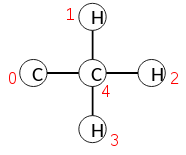
\includegraphics[height=3.3cm,width=3.7cm]{images/graphs/C2H3.png}
    \caption{Pattern graph}
    \label{C2H3}
  \end{minipage}
  \begin{minipage}[t]{.5\textwidth}
  \centering
  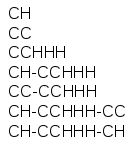
\includegraphics[height=3.9cm,width=3.8cm]{images/paths/C2H3-isomer-paths.png}
  \caption{Subtree-label paths}
  \label{C2H3-subtree-label-paths}
  \end{minipage}
\end{figure}
%%%%%%%%%%%%%%%%%%%%%%%%%%%%%%%%%%%%%%%%%%%%%%%%%%%%%%%%%%%%%%%%%%%%%%%%%%%%
\subsection{Algorithm Refinement}
  In order to solve the problem with false negatives, we changed the candidate extraction part. For every path $pp$ in the pattern index, we check which target graphs contain $pp$ as a path. Let us have $pp$ = \texttt{CH-CCHHH} and we want to check it against the target path $tp$ = \texttt{CH-CCCHHH-CHHH}. For every \textit{neighborhood label} in $pp$, our algorithm will whether it is contained in the corresponding label in $tp$. We first compare \texttt{CH} and \texttt{CH}, and as they are equal, we continue with the labels on the next position: \texttt{CCHHH} and \texttt{CCCHHH}. As \texttt{CCCHHH} contains \texttt{CCHHH} and this is the last label in $pp$, we stop and return true, $tp$ contains $pp$.\par
%%%%%%%%%%%%%%%%%%%%%%%%%%%%%%%%%%%%%%%%%%%%%%%%%%%%%%%%%%%%%%%%%%%%%%%%%%%%
Using the refinement described above, we removed the problem with false negatives, described in section \ref{path-subtree index problems}. However, this results in weaker filtering power. Now, there are some cases where $path$-$index$ would perform better, although it extracts less structural information about the graphs. We will show how our refined method introduces more false-positives using an example. Let us consider the two graphs on figures \ref{C2H4-1} and \ref{C2H}. Let us apply the refined $Path$-$Subtree$ indexing method for the two graphs, where \ref{C2H} is the pattern and \ref{C2H4-1} is the target (clearly, \ref{C2H4-1} does not contain \ref{C2H} as subgraph). The \textit{neighborhood labels} of the target and the pattern for $maxL$=3 are shown on figures \ref{C2H4-1-subtree-label-paths} and \ref{C2H-subtree-label-paths} respectively. Applying the new candidate extraction technique, we will have \ref{C2H4-1} returned as candidate, because it contains all paths in \ref{C2H}.\par
%%%%%%%%%%%%%%%%%%%%%%%%%%%%%%%%%%%%%%%%%%%%%%%%%%%%%%%%%%%%%%%%%%%%%%%%%%%%  
\begin{figure}[h]
\centering
\begin{minipage}[t]{.5\textwidth}
  \centering
  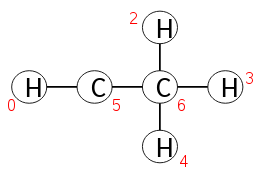
\includegraphics[height=3.3cm,width=4.4cm]{images/graphs/C2H4-1.png}
  \caption{Graph A}
  \label{C2H4-1}
\end{minipage}%
\begin{minipage}[t]{.5\textwidth}
  \centering
  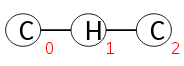
\includegraphics[height=1cm,width=3cm]{images/graphs/C2H.png}
  \caption{Graph B}
  \label{C2H}
\end{minipage}%

\begin{minipage}[t]{.5\textwidth}
  \centering
  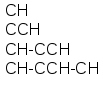
\includegraphics[height=4.4cm,width=3.9cm]{images/paths/C2H-isomer-paths.png}
  \caption{Neighborhood label paths of A}
  \label{C2H4-1-subtree-label-paths}
\end{minipage}%
\begin{minipage}[t]{.5\textwidth}
  \centering
  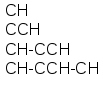
\includegraphics[height=2.1cm,width=2.7cm]{images/paths/C2H-isomer-paths.png}
  \caption{Neighborhood label paths of A}
  \label{C2H-subtree-label-paths}
\end{minipage}%
\end{figure}
%%%%%%%%%%%%%%%%%%%%%%%%%%%%%%%%%%%%%%%%%%%%%%%%%%%%%%%%%%%%%%%%%%%%%%%%%%%%
Let us examine in more detail the only path of length 3 in the pattern graph. It is composed from the nodes with ids \texttt{0, 1} and \texttt{2}. Using $Path$-$Subtree$ index method, this path is represented as \texttt{CH-CCH-CH} in the index file. If we used $path$-$index$, we would store this path as the string \texttt{C-H-C}. Although the path representation \textit{neighborhood label} gives us more information about the node neighbors, with us we loose important structural information, which is: the label of the actual node. In the string \texttt{CCH},  either of the letters could be the label of the node. As shown in the example above, this confusion leads to more false positives.\par
%%%%%%%%%%%%%%%%%%%%%%%%%%%%%%%%%%%%%%%%%%%%%%%%%%%%%%%%%%%%%%%%%%%%%%%%%%%%
TODO
  - we changed the string representation of the isomer label. First letter is always the original label, the others are from the neighbors, sorted in lexicographic order\\

\subsection{Implementation}
       
       - extend IB-Index 1 and put an option to extract paths using isomer labels.\\
       - describe the extension of the project to support both types of indexing.\\
       - when parsing the graphs, after parsing each graph, compute the isomer label of every node for this graph\\
       - additional field in Node class for isomer labels\\
       - we have a class Path to represent the paths. Each path is an array of nodes. There is a toString method that returns the desired string that we are to store in the index. Depending on the option, we can return path from the labels (ib-index 1), path from the isomer labels (ib-index 2) or a path from the id of each node, made for testing purposes There is a method to reverse the path and it is used when storing the paths in the index: we always store the lexicographically smaller path, comparing each path with its reversed equivalent.\\
       - re-written the candidates extraction part. We have to check for containment ... \\

 
 
 
%%%%%%%%%%%%%%%%%%%%%%%%%%%%%%%%%%%%%%%%%%%%%%%%%%%%%%%%%%%%%%%%%%%%%%%%%%%%
%%%------------------------------SIP Algorithms--------------------------%%%
%%%%%%%%%%%%%%%%%%%%%%%%%%%%%%%%%%%%%%%%%%%%%%%%%%%%%%%%%%%%%%%%%%%%%%%%%%%%

%% todo
%% remove sip0 and make sip1 be sip 0
%% make the graphs be in log scale
\chapter{Light Filters}
\label{ch:sip1}
This section describes the study of a simple \gls{sip} algorithm, called SIP1, that implements a fast filter that does not employ an index structure.

Light Filters is an algorithm for subgraph query processing and it is based on a modified version of the filter-verification paradigm. Here, filtering and verification steps are applied separately for each \gls{sip} instance. This approach uses simple filtering tests that require much less computational effort (i.e. lighter filtering). More importance is placed on the quality of the \gls{sip} algorithm than on the filters, because the major computational effort goes for solving the non-filtered \gls{sip} instances. 

Algorithm \ref{algo:roughSIP} is a pseudocode of our method. Given a file with targets T and a file with patterns P, we first read in each graph (lines 2, 3). Filtering is performed for every (G$_{p}$, G$_{t}$) pair and if the instance is not rejected, a call to \gls{sip} algorithm is made (line 7). The filter step consists of 5 naive tests, performed before the call to SIP1. If the conditions of any of the tests are not met, search does not proceed and we consider this to be a \textit{trivial fail}. 

Each step of the Light Filters algorithm is explained thoroughly. First, we introduce the theory behind the trivial fails and their implementation in Section \ref{sec:trivialFails}. We then introduce the SIP algorithm called SIP1 and discuss its implementation in Section \ref{sec:sip1}. Evaluation of the light filters approach is described in Chapter \ref{ch:evaluation}.

%%% light filters sip algorithm
\begin{algorithm}
\centering
\caption{Light filters algorithm}
\label{algo:roughSIP}
\begin{algorithmic}[1]
\Procedure{Process }{File p, File t} \Comment{\textit{file with patterns and file with targets}}
\State T$_{list}$ $\gets$ read in all targets from file, initialize objects
\State P$_{list}$ $\gets$ read in all patterns from file, initialize objects
\For{G$_{p}$ in P$_{list}$}
	\For{G$_{t}$ in T$_{list}$}
		\If{!\Call{Filter }{G$_{p}$, G$_{t}$}} \Comment{\textit{If the instance is not rejected during filtering, perform verification}}
    		\State{\Call{SIP1}{G$_{p}$, G$_{t}$}}
    	\EndIf
    \EndFor
\EndFor
\EndProcedure
\end{algorithmic}
\end{algorithm}
%%%% end of algorithm

\section{Trivial Failures}
\label{sec:trivialFails}

This Section introduces the five trivial failure tests, implemented as part of the filtering stage of SIP1.

\subsection{Neighborhood Degree Sequence}
\label{sec:nds}
The neighbourhood degree sequence of G and the degree sequence of labels in G correspond to four of the trivial tests. Very similar approach of using the degree sequence of vertices to reject \gls{unsat} \gls{sip} instances is used in the filtering part of the algorithm presented in \cite{Solnon:2010}.
 
\begin{definition}[Label Degree Sequence]
The \textit{\gls{lds}} of \textit{l} $\in$ L$_{G}$, denoted as $\gls{lds}$(G, \textit{l}) is the non-increasingly ordered list of the degrees of all vertices in V$_{G}$ that have \textit{l} assigned as their label.    
\end{definition}

\begin{definition}[Neighborhood Degree Sequence]
The \textit{\gls{nds}} of G, written as $\gls{nds}$(G), is the list of tuples (\textit{l}, $\gls{nds}$(\textit{l})) for every \textit{l} $\in$ L$_{G}$.
\end{definition}

\begin{example}
Let us have a graph G with two labels: A and B, where \gls{lds}(A) = \{5, 4, 3, 2, 2\} and \gls{lds}(B) = \{4, 3, 3, 1\}. This shows us that the order of G is 9, where 4 vertices with degrees 4, 3, 3 and 1 are labeled as B and 5 vertices with degrees 5, 4, 3, 2 and 2 are labeled as A. Using \gls{lds}, we derive that \gls{nds}(G) = \{\{A, \{5, 4, 3, 2, 2\}\}, \{B, \{4, 3, 3, 1\}\}\}.
\end{example}

\begin{definition}[G$_{t}$ subsumes G$_{p}$]
\label{def:subsumes}
We say that G$_{t}$ subsumes G$_{p}$ if for each label l both in G$_{p}$ and G$_{t}$, the length of the \gls{lds}(l$\in G_{p}$) is smaller or equal to the length of \gls{lds}(l$\in G_{t}$), and the degree on i$^{th}$ position in \gls{lds}(l$\in G_{p}$) is less than or equal to \gls{lds}(l$\in G_{t}$) for each i between 0 and $|\gls{lds}(l\in G_{p})|$.
\end{definition}

The notion of \gls{nds} lets us define several simple tests for incompatibility between \gls{pattern} and \gls{target}, based on checking whether \gls{nds}(G$_{p}$) is a subset of \gls{nds}(G$_{t}$). \gls{nds}(G$_{p}$) $\subseteq$ \gls{nds}(G$_{t}$) if all following conditions are true:
\begin{enumerate}
\item the order of G$_{p}$ is less than or equal to the order of G$_{t}$
\item the number of unique labels in G$_{p}$ is less than or equal to the number of unique labels in G$_{t}$
\item every label in G$_{p}$ is also in G$_{t}$
\item G$_{t}$ subsumes G$_{p}$
\end{enumerate}

\begin{example}
Let us have \gls{nds}(G$_{p}$) = \{\{A, \{3, 2, 1\}\}, \{B, \{4\}\}\} and
\gls{nds}(G$_{t}$) = \{\{A, \{5, 4, 3, 2, 2\}\}, \{B, \{4, 3, 3, 1\}\}, \{C, \{5, 4, 2, 1\}\}\}.

In this example, \gls{nds}(G$_{p}$) is a subset of \gls{nds}(G$_{t}$), because each of the four conditions is true. In particular:
\begin{enumerate}
\item The order of G$_{p}$ (4) is less than the order of G$_{t}$ (13).
\item The number of unique labels in G$_{p}$ = 2 and the number of unique labels in G$_{t}$ is 3. 3 is clearly bigger than 2.
\item G$_{p}$ has labels A and B which are both in G$_{t}$.
\item The \gls{lds} of every label in G$_{p}$ is clearly contained in the \gls{lds} of the same label in G$_{t}$.
\end{enumerate}
\end{example} 

\begin{theorem}
\label{th:nds}
If \gls{nds}(G$_{p}$) $\nsubseteq$ \gls{nds}(G$_{t}$), then \gls{sip}(G$_{p}$, G$_{t}$) is \gls{unsat}.
\end{theorem}

\begin{proof}
Suppose that \gls{sip} (G$_{p}$, G$_{t}$) is \gls{sat} and that \gls{nds}(G$_{p}$) $\nsubseteq$ \gls{nds}(G$_{t}$). Then, at least one of the conditions for \gls{nds}(G$_{p}$) $\subseteq$ \gls{nds}(G$_{t}$) is not true.
\begin{enumerate}
\item Suppose that the first condition is false. Then, G$_{p}$ must have at least one vertex more than G$_{t}$, i.e. at least one vertex $\in$ G$_{p}$ will be unmatched. Therefore, \gls{sip} (G$_{p}$, G$_{t}$) is \gls{unsat} if the order of G$_{p}$ is bigger than the order of G$_{t}$ and we reach a contradiction. Therefore, this condition must always hold.
\item Suppose that the second condition is false so that there exists a label l$^{\prime}$ $\in$ L$_{G_{p}}$ with l$^{\prime}$ $\notin$ L$_{G_{t}}$. Therefore, there exists a vertex \textit{v} $\in$ G$_{p}$ that is assigned the label l$^{\prime}$ and there is no vertex in G$_{t}$ with label l$^{\prime}$. From this follows that \textit{v} can not be matched to any vertex in G$_{t}$ and \gls{sip}(G$_{p}$, G$_{t}$) is \gls{unsat}, which leads to a contradiction. Therefore, condition 2 must hold.
\item Suppose that the third condition is false. Then, there exists a label l$^{\prime}$ $\in$ L$_{G_{p}}$ and l$^{\prime}$ $\notin$ L$_{G_{t}}$. As proved before, this is a contradiction, therefore condition 3 must hold.
\item Suppose that previous three conditions hold and G$_{t}$ does not subsume G$_{p}$.

First, suppose that for each label l both in G$_{p}$ and G$_{t}$, the length of the \gls{lds}(l$\in G_{p}$) is smaller or equal to the length of \gls{lds}(l$\in G_{t}$). Then, there exists a degree value \textit{deg$_{pi}$} $\in$ \gls{lds}(l$\in G_{p}$) at position \textit{i} in the list for \textit{i} between 1 and $| \gls{lds}(l\in G_{p})|$ such that \textit{deg$_{pi}$} $>$ \textit{deg$_{ti}$}, where \textit{deg$_{ti}$} $\in$ \gls{lds}(l$\in G_{t}$). Then, there is a vertex \textit{v} $\in$ G$_{p}$ with label l and degree \textit{deg$_{pi}$} that will not be matched to any vertex in G$_{t}$. Therefore \gls{sip} (G$_{p}$, G$_{t}$) is \gls{unsat} which is a contradiction, therefore the degree of the \textit{i$^{th}$} element in \gls{lds} of each label in G$_{p}$ has to be smaller or equal to the degree of the \textit{i$^{th}$} element for the corresponding label in G$_{t}$ for every \textit{i} between 0 and the length of \gls{lds} of every label in G$_{p}$.

Second, suppose that there exists a label l both in G$_{p}$ and G$_{t}$ such that the length of the \gls{lds}(l$\in G_{p}$) is bigger than the length of \gls{lds}(l$\in G_{t}$). Then, the number of vertices with label l in G$_{p}$ is bigger than the number of vertices with label l in G$_{t}$ and it is impossible to match each vertex in G$_{p}$ to a different vertex in G$_{t}$ which leads to contradiction.

Therefore both conditions of subsumption must hold and G$_{t}$ subsumes G$_{p}$. This is a contradiction, therefore condition 4 must be true.
\end{enumerate} 

All four conditions must hold. It follows that \gls{nds}(G$_{p}$) $\subseteq$ \gls{nds}(G$_{t}$) which is a contradiction. Therefore, if \gls{nds}(G$_{p}$) $\subseteq$ \gls{nds}(G$_{t}$), then \gls{sip}(G$_{p}$, G$_{t}$) is \gls{unsat}.
\end{proof}

The four conditions for \gls{nds}(G$_{p}$) $\subseteq$ \gls{nds}(G$_{t}$) are the first four of the trivial failures added to SIP1, also displayed on Table \ref{table:failures}. Their implementation is discussed in Section \ref{sec:trivialFailsImplementation}.

\subsection{Domain wipe out}
\label{sec:domainWipeout}
This is the fifth of the trivial failures implemented as light filtering on top of the search. Every pattern vertex \textit{v} has a bitset domain \textit{dom$_{v}$}. The size of \textit{dom$_{v}$} is equal to the order of the target, where every bit corresponds to a vertex in the target. For every vertex \textit{w} $\in$ G$_{t}$, if L(\textit{w}) is equal to L(\textit{v}) and the degree of \textit{v} is smaller or equal to the degree of \textit{w}, we set the bit for \textit{w} in \textit{dom$_{v}$} to true, i.e. \textit{v} can be mapped to \textit{w}. Whenever no bit in \textit{dom$_{v}$} is set to 1, it means that no target vertex exists that can be mapped to \textit{v} i.e. no valid mapping from all vertices in G$_{p}$ to a different vertex in G$_{t}$ can exist and \gls{sip} (G$_{p}$, G$_{t}$) is \gls{unsat}. The algorithm returns false without proceeding to search.

Table \ref{table:failures} shows the trivial failures discussed. They are executed as tests in the same hierarchy as shown in the Table. The first four failures are namely the conditions for \gls{nds}(G$_{p}$) $\subseteq$ \gls{nds}(G$_{t}$). If either of these tests fails, then \gls{sip}(G$_{p}$, G$_{t}$) is \gls{unsat} (Theorem \ref{th:nds}).

\subsection{Order of Tests}

Tests follow a strict hierarchy, where test 1 performs the cheapest and most trivial task and test 5 is the most expensive and its filtering is based on the least trivial test. The cost of each test in terms of complexity is discussed in Section \ref{sec:trivialFailsImplementation}.

%%% todo: make a discussion about the dependency between these failures, i.e. what happens if we switch off one failure or not. Write an informal proof about it?

%\begin{itemize}
%\item Filter 2 and 3 filter differently. Ex: p = \{A,B,B,C\} and t=\{A,B,C\}. Test 2 passes, but test 3 fails
%\end{itemize}

%%%% table about failures %%%%
\begin{table}
\centering
\renewcommand{\arraystretch}{1.5}% Spread rows out...
\begin{tabular}{ >{\centering\bfseries}m{1in} >{\centering\arraybackslash}m{2.3in}} 
\toprule
  Trivial Fail & Meaning\\
\midrule
 \textbf{1} & G$_{t}$.order $\geq$ G$_{p}$.order\\
 \rowcolor{Gray}
 \textbf{2} & G$_{t}$ unique labels $\geq$ G$_{p}$ unique labels\\
 \textbf{3} & G$_{p}$ labels $\subseteq$ G$_{t}$ labels\\
 \rowcolor{Gray}
 \textbf{4} & G$_{t}$ subsumes G$_{p}$\\
 \textbf{5} & \textit{dom$_{v}$}, \textit{v} $\in$ G$_{p}$ not empty\\
 \bottomrule
\end{tabular}
\caption{Specification of the measured failure types}
\label{table:failures}
\end{table}        
%%%%

\subsection{Implementation}
\label{sec:trivialFailsImplementation}
Algorithm \ref{algo:filters} describes the implementation of the 5 trivial failures from Table \ref{table:failures} as part of the filtering stage. Procedure ``filter'' is executed for every \gls{sip} instance before the verification stage. If any of the if statements (lines 2, 4, 6, 8 and 17) is false, the procedure returns false and the verification for the corresponding instance is not executed. Otherwise, if all 5 tests are true, the procedure makes a call to SIP1, i.e proceeds to the verification step. Pseudocode for SIP1 is shown in Algorithm $say where$ and discussed in the next Section.

%% comment on the expensiveness of each trivial failure
Failures 1 and 2 are the fastest: each of them takes time $\mathcal{O}(1)$ to compute. For failure 1, one needs only to return the sizes of the number of vertices in G$_{p}$ and in G$_{t}$. For failure 2, for every graph G, we have an array that stores all unique labels that occur in G. The size of this array is known after the graph is read from the file. To check whether test 2 is true, one needs to compare the size of the labels array d$_{p}$ of G$_{p}$ with the size of the labels array d$_{t}$ of G$_{t}$. Finding the values of d$_{t}$ and d$_{p}$ takes time $\mathcal{O}(1)$.

Failures 3 and 4 have slower running time. For every label l $\in$ G$_{p}$, failure 3 occurs if l is not a label in G$_{t}$. Checking whether l is a label in G$_{t}$ involves iterating over the labels in G$_{t}$, which is of time $\mathcal{O}(d_{t})$ worst case, if l is the last label in G$_{t}$ or it is not present. Therefore, the overall complexity of failure 3 is $\mathcal{O}(d_{p}.d_{t})$. Algorithm \ref{algo:subsumes} shows the pseudo code for the ``subsumes'' procedure. Its complexity is $\mathcal{O}(plds)$, where plds is the \gls{lds} of label \textit{l} $\in$ G$_{p}$. Therefore, the overall complexity of failure 4 is $\mathcal{O}(plds.d_{p})$.

Failure 5 is the most expensive one. It takes time $\mathcal{O}(m.n)$, where n is the order of G$_{p}$ and m is the order of G$_{t}$. Algorithm \ref{algo:filters} has to visit each vertex \textit{v} $\in$ G$_{p}$, initialize dom$_{v}$ and for every \textit{w} $\in$ G$_{t}$, check whether \textit{w} can be mapped to \textit{v}. The two checks (line 13) take time $\mathcal{O}(1)$.

%% failures algorithm
\begin{algorithm}
\centering
\caption{Lights Filters}
\label{algo:filters}
\begin{algorithmic}[1]
\Procedure{Filter }{G$_{p}$, G$_{t}$}
\If {\textbf{not} G$_{t}$.order $\geq$ G$_{p}$.order} \Return false \Comment{\textit{trivial failure 1}}
\EndIf
\If {\textbf{not} G$_{t}$ unique labels $\geq$ G$_{p}$ unique labels} \Return false \Comment{\textit{trivial failure 2}}
\EndIf
\For {\textit{l} in L$_{G_{p}}$}
%\State{
	\If {\textbf{not} \textit{l} in L$_{G_{t}}$} \Return false \Comment{\textit{trivial failure 3}}
	\EndIf
	\If {\textbf{not}  \Call{subsumes }{G$_{p}$, G$_{t}$, \textit{l}}} \Return false \Comment{\textit{trivial failure 4}}
	\EndIf
%}
\EndFor
\State alldoms $\gets$ initialize \Comment{\textit{An array of size the order of G$_{p}$ that contains the domain of each vertex in G$_{p}$}}
\For{every \textit{v} $\in$ G$_{p}$}
\State{
	dom$_{v}$ = new BitSet(G$_{t}$.order) \Comment{\textit{initialize dom$_{v}$ to bitset of size the order of the target}}
	\For{every \textit{w} $\in$ G$_{t}$}
    	\If {\textit{v}.label == \textit{w}.label \textbf{and} \textit{v}.degree $\leq$ \textit{w}.degree}
        \State {set dom$_{v}$[\textit{w}] to 1}
        \EndIf
	\EndFor \\
    alldoms[v] $\gets$ dom$_{v}$
	\If {empty \textit{dom$_{v}$}} \Return false \Comment{\textit{trivial failure 5}}
}
\EndFor \\
\Call{sip1}{alldoms} \Comment{\textit{if no failures occurred, call SIP1 algorithm}}
\EndProcedure
\end{algorithmic}
\end{algorithm}
%%% end of algorithm

%%% subsumes
\begin{algorithm}
\centering
\caption{G$_{t}$ Subsumes G$_{p}$}
\label{algo:subsumes}
\begin{algorithmic}[1]
\Procedure{subsumes }{G$_{p}$, G$_{t}$, \textit{l}}
\State plds $\gets$ lds(l) in G$_{p}$ \Comment{\textit{the label degree sequence of l in G$_{p}$}}
\State tlds $\gets$ lds(l) in G$_{t}$ \Comment{\textit{the label degree sequence of l in G$_{t}$}}
\For{i between 0 and pSeq.length - 1}
\If {plds[i] $>$ tlds[i]} \Return false \Comment{\textit{exists vertex in G$_{p}$ that can`t' be matched to any vertex G$_{t}$}}
\EndIf
\EndFor \\
return true
\EndProcedure
\end{algorithmic}
\end{algorithm}
%%% end of subsumes
For the implementation of the filtering, the following classes are introduced.

\begin{itemize}
\item Class Graph\\
Creates \gls{graph} from a file. A Graph object has size, order, id, array of the degree of each vertex, bitset array of the neighbours of each vertex, where the i$^{th}$ element in the array contains the neighbours of vertex i in the graph and array of labels, where similarly, the element in position i contains the label of vertex i. While reading in the graph, we initialize each field, which takes time $\mathcal{O}(size+order)$. When the array of labels is built, a new object for each unique label \textit{l} is created and the \gls{nds} of the graph is computed.
\item Class Label\\
This class represents a label in a Graph object. A Label has a name and \gls{lds} which is an array of integers, sorted in non-increasing order. The degree sequence array is built using insertion sort algorithm which is of complexity $\mathcal{O}(n^{2})$, where n is the size of \gls{lds} \cite{Cormen:2001:IA:580470}.
\item Class SIP1\\
This class implements the light filtering procedure displayed in Algorithm \ref{algo:filters} as well as the \gls{sip} algorithm, which is explained in more detail in the next Section.
\end{itemize}

\section{SIP1 Implementation}
\label{sec:sip1}
SIP1 is based on the simplest of the Glasgow algorithms \cite{CP2015}. Given a \gls{pattern} and \gls{target}, SIP1 has a variable for each vertex in \gls{pattern}, each with domain that is the set of compatible vertices in \gls{target} (alldoms, Algorithm \ref{algo:sip1}, initialized in Algorithm \ref{algo:filters}). Compatible vertices have the same labels and the degree of the target vertex is greater than or equal to the degree of the pattern vertex. Bit sets are used to represent the domains and the adjacency matrices of the graphs. When a pattern variable $u$ is instantiated with a target value $i$ (Algorithm \ref{algo:sip1}, line 7), all uninstatiated (future) variables have $i$ removed from their domains (Algorithm \ref{algo:sip1}, line 12). If a future variable $v$ is adjacent to $u$ in \gls{pattern} then the domain of $v$ becomes the intersection of the current domain of $v$ with the neighborhood of vertex $i$ in \gls{target}. This constraint is enforced by applying a logical $and$ operation between the two bit sets (Algorithm \ref{algo:sip1}, line 14). SIP1 uses \gls{forwcheck} with fail first heuristic \cite{haralickElliot:1980}: for all uninstantiated variables representing pattern vertices, it selects to explore the one that has the smallest domain before the others (Algorithm \ref{algo:sip1}, line 4).

Class SIP1 contains the implementation of the verification step. For every \gls{sip}(G$_{p}$, G$_{t}$) instance, if it is not discarded after filtering, it goes to the SIP1 procedure (line 21, Algorithm \ref{algo:filters}). Algorithm \ref{algo:sip1} is a pseudocode of the implementation.

%%% SIP1 pseudocode
\begin{algorithm}
\centering
\caption{SIP1 }
\label{algo:sip1}
\begin{algorithmic}[1]
\Procedure{SIP1 }{alldoms}
\If{alldoms is empty} \Return solution \Comment{\textit{true or false}}
\EndIf
\State dom$_{u}$ $\gets$ smallest(alldoms) \Comment{\textit{select vertex u with the smallest domain first}}
\State newAlldoms $\gets$ initialize with size=(alldoms.size - 1)
\For{i in dom$_{u}$.getNextSetBit} \Comment{\textit{for each entry in u with bit set to 1}}
	\State assign i as a value of vertex u
	\For{(dom$_{v}$ in alldoms) $\land$ (dom$_{v}$ != dom$_{u}$)} \Comment{\textit{the domain of each vertex}}
		\If{!consistent} \Return consistent $\land$ \Call{SIP1}{newAlldoms} 
        \EndIf
        \State newdom$_{v}$ $\gets$ dom$_{v}$
        \State set i$^{th}$ entry of newdom$_{v}$ to false \Comment{\textit{cannot take value assigned to u}}
        \If{u is adjacent to v in G$_{p}$}
        	\State (newdom$_{v}$)AND(neighbours of i in G$_{t}$) \Comment{\textit{v can only take vertices in G$_{t}$ adjacent to i}}
        \EndIf
        \State add newdom$_{v}$ to newAlldoms
        \State consistent $\gets$ !(newdom$_{v}$ == 0) \Comment{\textit{if there is a domain wipe out, consistent becomes false}}
	\EndFor
    \State consistent $\land$ \Call{SIP1}{newAlldoms}
\EndFor
\EndProcedure
\end{algorithmic}
\end{algorithm}
%%% end of SIP1 pseudocode
In the worst case, SIP1 will assign all values from the domain of each pattern vertex, making recursive calls to SIP1 and failing late, therefore exploring very deep in the search tree before finding that there is no solution. In practice, due to the fail first heuristic used, the algorithm very rarely fails deep in the search tree, because the value that is most likely to fail is first explored, therefore failures occur mostly near the top of the search tree. 

\chapter{Evaluation}
\label{ch:evaluation}

%\section{Empirical study of path-based filtering}
%\subsection{Performance}
%TODO \\
%       - the index file is bigger, but the candidate set is smaller\\
%       - put the table with results\\
%       - explain the results and why they are like this\\
%	   - complexity?\\
% 	   - what could be done better and how?\\

%\subsection{Variants of Path-Subtree index}
%TODO \\
 %- use neighborhood of length 2, 3 ...
 %- this will result in bigger index, but even stronger filtering strength, which means

%\subsection{Advantages and Limitations}
%TODO \\
% - very easy to implement, especially when we have index-1 implementation ready\\
 %- the index file is even bigger --- this is  bad\\
 

%%% TODO make graphs with the running time in milliseconds
\section{Light Filters}
\label{eval:sip1}
This Section reports on the observed performance of the subgraph query processing algorithm described in Chapter \ref{ch:sip1}. SIP1 was run with each of the datasets discussed in Section \ref{sec:datasets}, some of which were also used for empirical study by \cite{foteini, graphgrepsx, GRAPES, graphgrepsx, ctindex, gcode, tree+delta>=graph}. The experiments are conducted on a Windows 7 SP1 host with 2 Intel Xeon E5-2660 CPUs (2.20GHz, 20MB Cache, 8 cores/16 threads per CPU) and 128GB of RAM, same machine used by \cite{foteini}. Run time is measured in milliseconds from when the process starts until it completes, including the time to read in all the graphs, to perform filtering and verification for each instance and to write out all results to a file.

For each rejected \gls{sip} instance during filtering, we recorded the test that rejected it using the scale on Table \ref{table:failures} and calculated the total number of instances that were eliminated by a particular test for each dataset. These numbers were then used to derive the percentage of \gls{sip} instances eliminated by each fail test. We also computed the percentage of \gls{sat} and \gls{unsat} \gls{sip} instances for each dataset. Figure \ref{averageFailures} shows our results. The brown part of each bar represents the percentage of \gls{sip} instances that are \gls{sat}, the rest of the bar for \gls{unsat} problems. All satisfiable instances had to go through the verification step, whereas for some of the \gls{unsat} problems were discarded during the filtering. For instance, the leftmost bar represents the aids dataset, where 8.67\% of all instances are \gls{sat}. Out of the \gls{unsat} problems, 24.211\% were discovered during the verification stage and the rest 32.881\% were filtered by either of the trivial failures. The number of \gls{sat} and \gls{unsat} problems are on Table \ref{table:dataSAT}. The following observations were made:

\begin{itemize}
\item Filtering gives best performance for the instances in the aids dataset. In particular, almost 70\% of the targets are rejected before verification. Aids also contains the largest number of \gls{unsat} instances. Also, this dataset tends to be the main one (and sometimes the only one) used for evaluation for some subgraph query processing algorithms like \cite{graphgrepsx, ctindex, gcode, tree+delta>=graph}.

\item Filtering is not successful for any instance in pdbs. Similarly, only 3.75\% of the targets were filtered in ppigo. In other words, \gls{sip} call was made for every pattern and target graph in the dataset, because they were compatible with respect to every condition on table \ref{table:failures}. The main reason is that most of the instances of pdbs and ppigo are \gls{sat} (77.22\% and 61\% respectively) and had to go through verification to be solved. Here, filtering can be effective for at most 22.78\% and 39\% of the instances. In such cases, query processing method that puts low amount of effort (or none) during filtering and implements an efficient verification algorithm will show much higher performance than method that employs heavy filtering approach and naive \gls{sip} algorithm for verification. This hypothesis was confirmed by the results of the study presented in \cite{foteini}, where each of the evaluated heavy indexing techniques, evaluated using the same datasets, demonstrated several times poorer performance than the light filtering technique discussed here.

\item There are duplicate target graphs in the pcms and pdbs datasets. The pcms database is supposed to contain 200 targets \cite{datasets}. In practice, there are only 50 unique graphs and each of them is added 4 times. The pdbs dataset is composed of 600 targets \cite{datasets}, but out of them only 30 are unique, each of them duplicated 20 times.
\end{itemize}

%%% 
\begin{figure}[H]
\centering
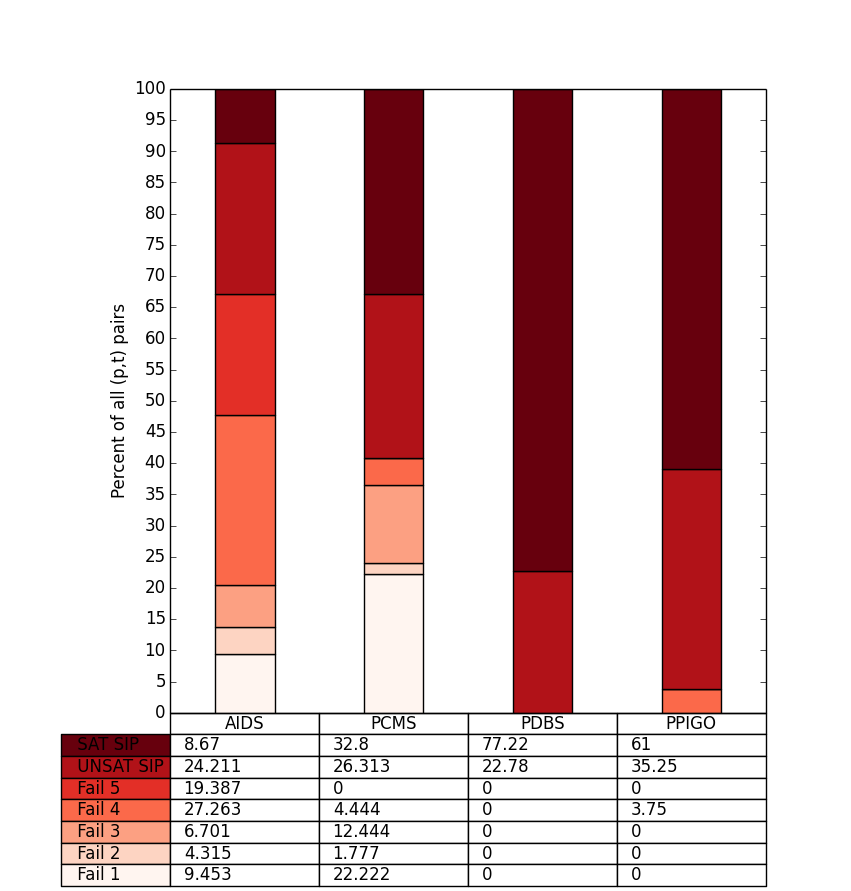
\includegraphics[height=15cm,width=13.5cm]{images/plots/splittedSIP.png}
\caption{Satisifability and average filtering percentage for each method in Table \ref{table:failures} for each of the datasets}
\label{averageFailures}
\end{figure}
%%%

\subsection{Hardness of \gls{sip} in terms of search nodes}
We report on the cost of the verification step in terms of the number of \glspl{sn} taken to solve a \gls{sip} instance. A search node denotes the number of recursive \gls{sip} calls taken to find a solution if the problem is \gls{sat} or prove that the problem is \gls{unsat}. For every dataset T, we take all instances that were not rejected during filtering and we compute the number of search nodes taken to solve \gls{sip} for each instance. We then compute the number of instances $|T_i|$ solved in a given number of search nodes $i$ for $0$ $<$ $i$ $<$ $n_{max}$, where  $n_{max}$ is search nodes taken to solve the hardest \gls{sip} instance in T. Figures \ref{aidsNodes}, \ref{pcmsNodes}, \ref{pdbsNodes} and \ref{ppigoNodes} present our results. Here, $|T_i|$ is represented as percentile of all targets (the x-axis). The search effort is plotted, starting from the easiest percentile (the leftmost part of the x-axis) and finishing with the last percentile representing the hardest instances in terms of search effort (on the rightmost part of the x-axis). The y-axis shows the cumulative difficulty of SIP calls in terms of search nodes for each percentile of the targets in a log scale. For example, looking at Figure \ref{aidsNodes}, 24\% of the targets are solved by using at most 2 nodes of search and 50\% of all targets are solved in less than 10 nodes. The hardest instances take at most 600 nodes.

The value on the y-axis for each percentile of T represents the number of search nodes taken to solve the hardest instance that belongs to the percentile. In other words, the graphs below show the hardest instance observed for each percentile of T. For example, if we had 3 graphs that belong to the i$^{th}$ percentile of T and they were solved in 1, 2 and 10 nodes respectively, the y-axis value of i would be 10. Therefore, the datasets are in practice easier than what is shown on Figures \ref{aidsNodes}, \ref{pcmsNodes}, \ref{pdbsNodes} and \ref{ppigoNodes}, which present the hardest instance for each percentile in the dataset. These Figures help us to make the following observations:
\begin{itemize}
\item The easiest dataset is ppigo. Looking at Figure \ref{ppigoNodes}, 88\% of all targets are solved by using at most 4 search nodes, 28\% are solved by using at most 1 node of search effort. The hardest problem (the right-most bar) takes 65 nodes to solve and it is between pattern ``8\_1.6" and target ``\#MUS$/$Mus\_musculus.sif$>$0.5.sif". The time taken to solve this is 4 milliseconds and the instance is \gls{unsat}.

\item pdbs is harder than ppigo and aids with most varied number of search nodes per instance. It is on average harder than pcms, however, the hardest instance in pcms takes more search effort than the hardest instance in pdbs. Figure \ref{pdbsNodes} shows that 20\% of the targets in pdbs are solved by using at most 100 nodes, which is significantly higher than ppigo, where even the hardest instance was solved in less than 70 nodes. The hardest instance here is between pattern ``32$\_$1ARO" and target ``\#g" and it is solved in 7,152 nodes for 95 milliseconds. This instance is \gls{unsat}. 

\item The dataset with the hardest instance is pcms. The hardest SIP takes 10,470 nodes to solve and it is between pattern ``16\_1C5G.cm.A" and target ``1CY2.cm.A.cmap". It was solved in 12 milliseconds and it is unsatisfiable. Looking at the other 99\% of pcms targets, we can see that they are mostly easy. For example, 43\% of the SIP instances are solved by using at most 10 nodes of search effort.

\item The aids dataset is comparably easy. The maximum nodes taken to solve a SIP instance took 619 nodes of search effort. It is the SIP call between pattern \#1 and target \#629591, it took 0 milliseconds of time and it is \gls{unsat}.

\item Looking at aids, pcms and pdbs, the number of nodes taken to solve SIP grows exponentially with the percentile of the population.

\item The hardest instance of each dataset is \gls{unsat}.

\item All four datasets are easy.
\end{itemize}

%%%
\begin{figure}
\centering
\begin{minipage}[t]{.5\textwidth}
  \centering
  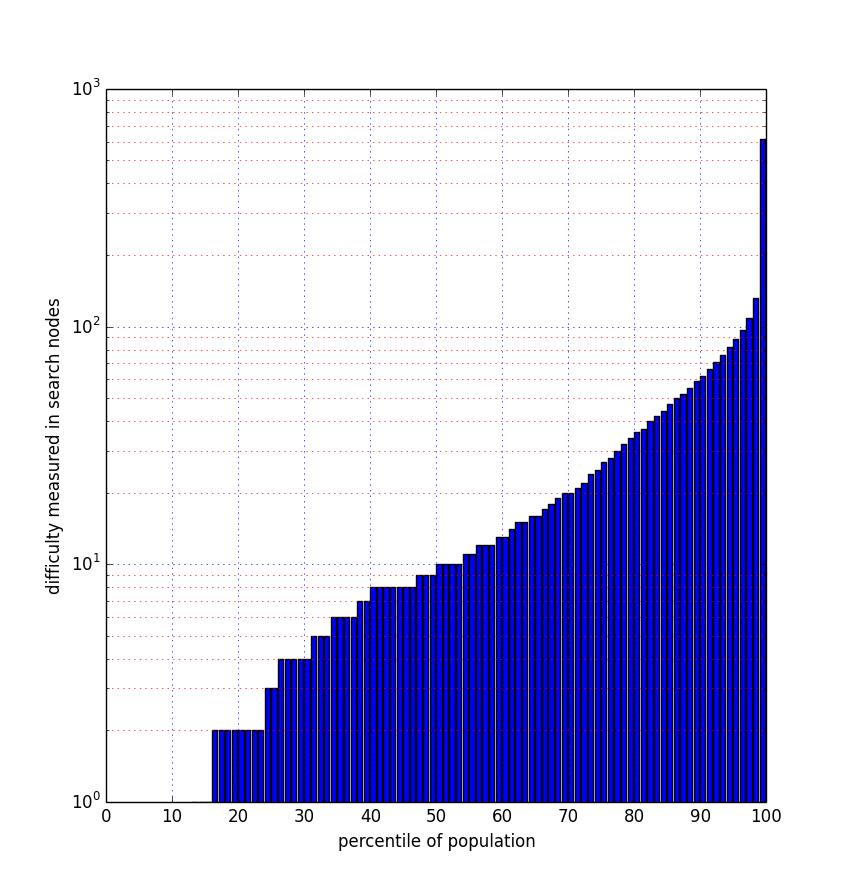
\includegraphics[height=11cm,width=9cm]{images/plots/aidsPercentileLog.png}
  \caption{SIP on aids dataset}
  \label{aidsNodes}
\end{minipage}%
\begin{minipage}[t]{.5\textwidth}
  \centering
  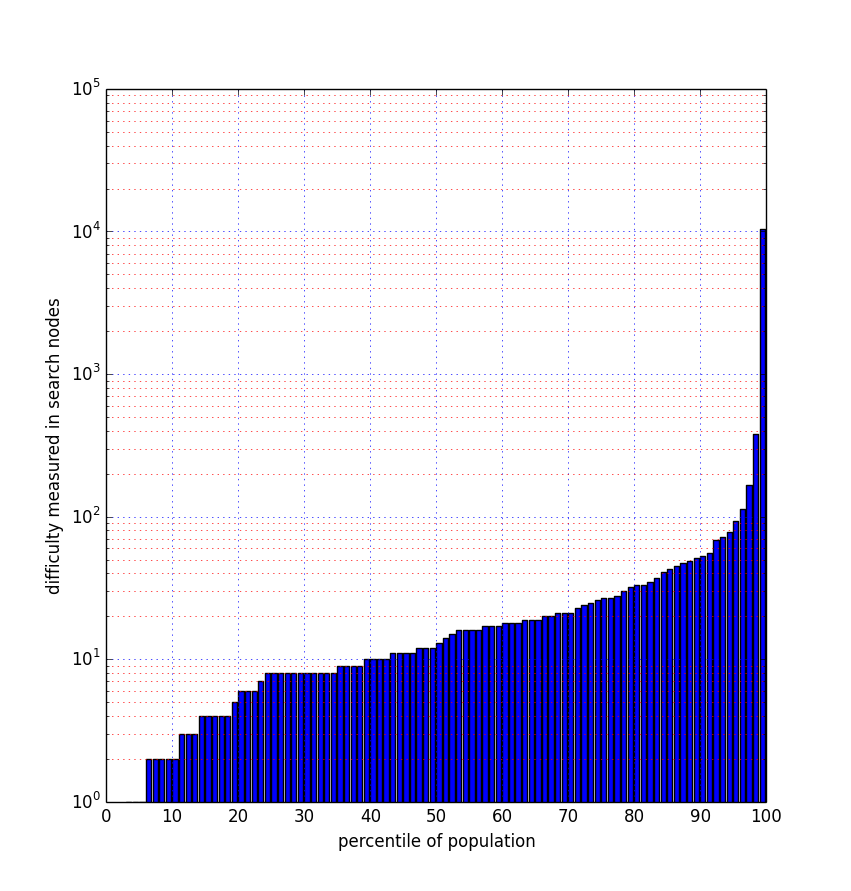
\includegraphics[height=11cm,width=9cm]{images/plots/pcmsPercentileLog.png}
  \caption{SIP on pcms dataset}
  \label{pcmsNodes}
\end{minipage}
\end{figure}
\begin{figure}
\centering
\begin{minipage}[t]{.5\textwidth}
  \centering
  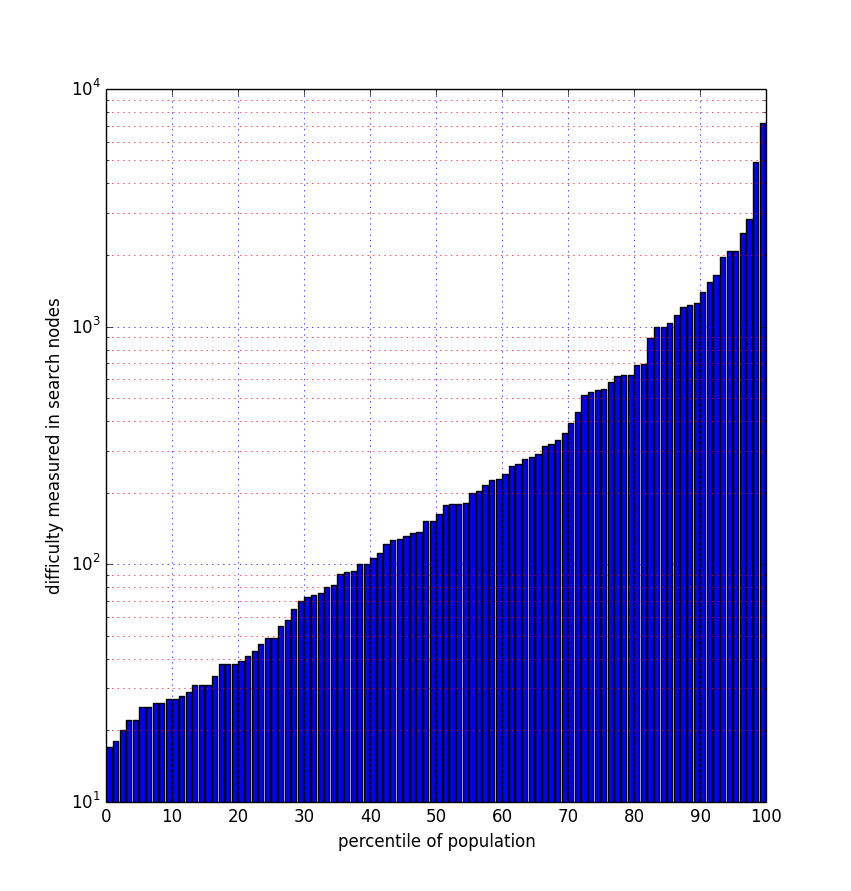
\includegraphics[height=11cm,width=9cm]{images/plots/pdbsPercentileLog.png}
  \caption{SIP on pdbs dataset}
  \label{pdbsNodes}
\end{minipage}%
\begin{minipage}[t]{.5\textwidth}
  \centering
  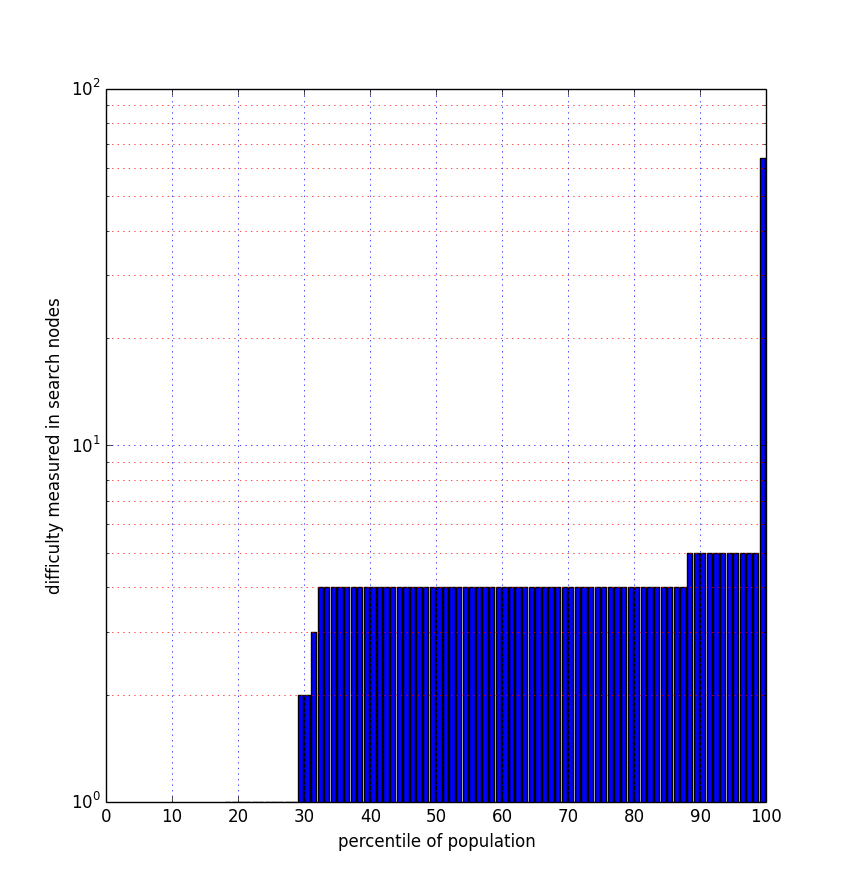
\includegraphics[height=11cm,width=9cm]{images/plots/ppigoPercentileLog.png}
  \caption{SIP on ppigo dataset}
  \label{ppigoNodes}
\end{minipage}
\end{figure}
%%%%

\subsection{Hardness of SAT vs UNSAT SIP instances}

The observation that the hardest instance of each dataset is unsatisfiable raises the following question: is \gls{unsat} \gls{sip} generally harder than SAT SIP? The experiments described in this section are again conducted in terms of number of search nodes and they are intended to further investigate this observation.

The following eight plots below break each of the plots discussed in the previous section (namely \ref{aidsNodes}, \ref{pcmsNodes}, \ref{pdbsNodes} and \ref{ppigoNodes}) further down in terms of whether the SIP instances are \gls{sat} or \gls{unsat}. The blue plots represent all satisfiable SIP pairs for a dataset D. Similarly, the red plots represent all unsatisfiable SIP instances of D. For each D (namely, for aids, pcms, pdbs and ppigo), the union of the blue plot (\gls{sat} \gls{sip}, left-hand side) and the red plot (\gls{unsat} \gls{sip}, right-hand side) gives the plot for the corresponding dataset discussed in the previous Section.

Note that the plots on Figure \ref{fig:ppigoSatUnsat} contain only 4 bars each, i.e. the data is divided into quartiles instead of percentile. Here, each bar represents 25\% of all instances of a category (\gls{sat}/\gls{unsat}). For example, the left plot shows that the lowest quartile of the \gls{sat} \gls{sip} calls takes no more than 4 nodes to solve, as it is also true for the second quartile. We changed the percentile representation for this dataset, because the number of \gls{sat} and \gls{unsat} \gls{sip} (61 and 39 respectively, Table \ref{table:dataSAT}) instances is too small to be scaled to percentiles.
%%% SAT vs UNSAT in terms of search nodes
\begin{figure}
\centering
\begin{minipage}[t]{.5\textwidth}
  \centering
  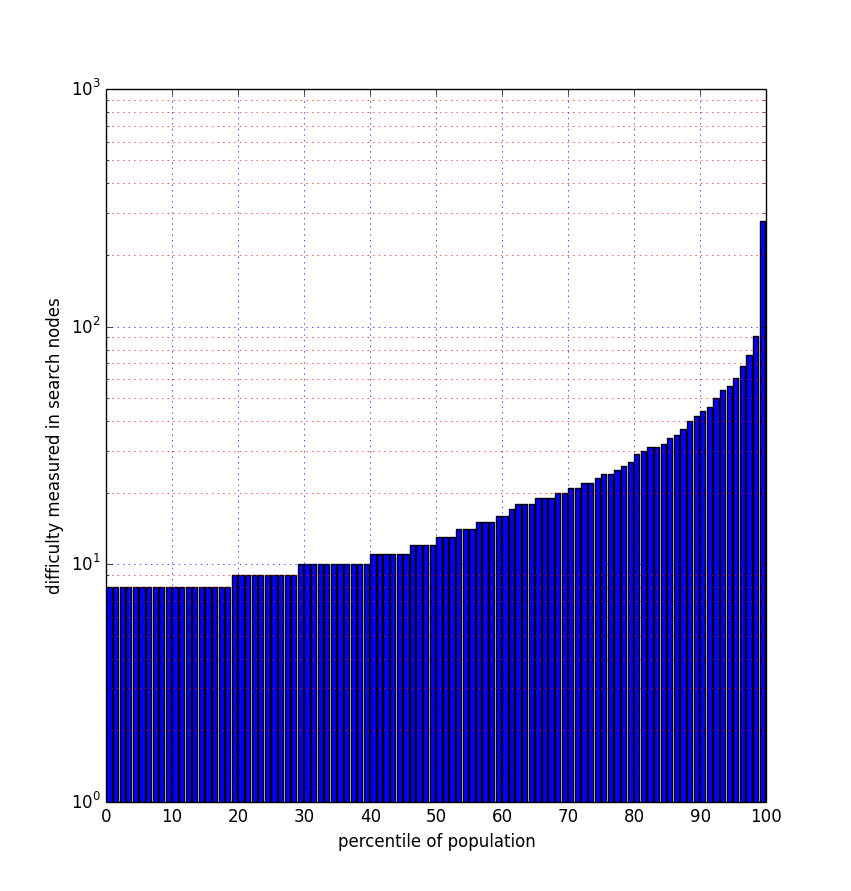
\includegraphics[height=11cm,width=9cm]{images/plots/aidsSAT.png}
\end{minipage}%
\begin{minipage}[t]{.5\textwidth}
  \centering
  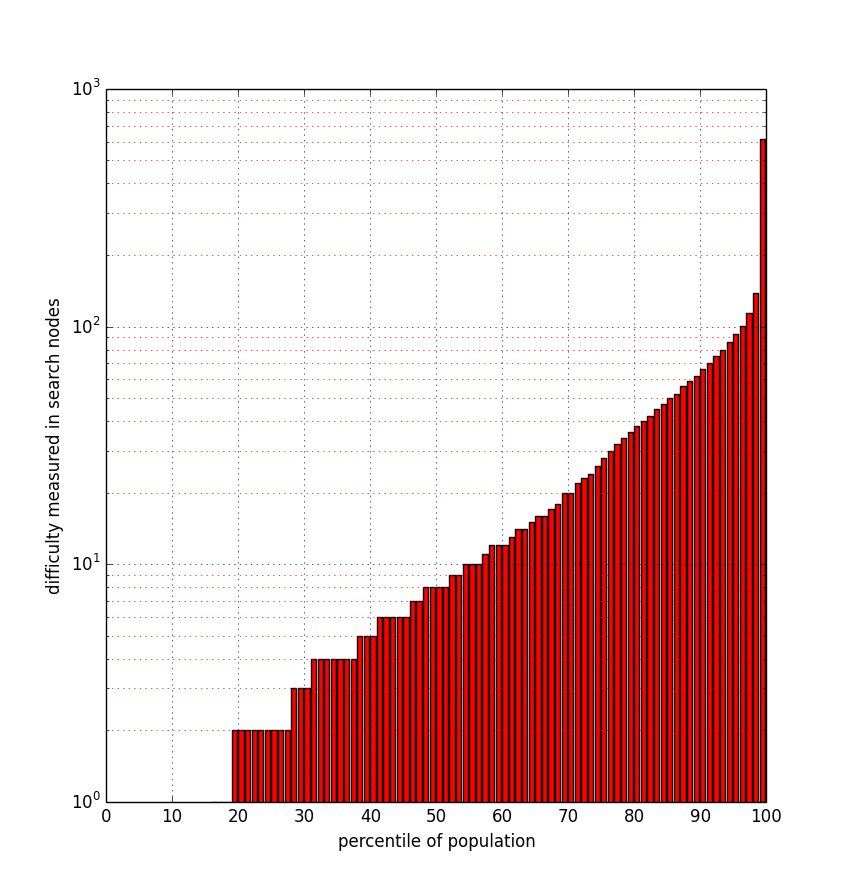
\includegraphics[height=11cm,width=9cm]{images/plots/aidsUNSAT.png}
\end{minipage}
\caption{Search effort for \gls{sat}(blue, left) \gls{unsat}(red, right) \gls{sip} instances in aids}
\label{fig:aidsSatUnsat}
\end{figure}
\begin{figure}
\centering
\begin{minipage}[t]{.5\textwidth}
  \centering
  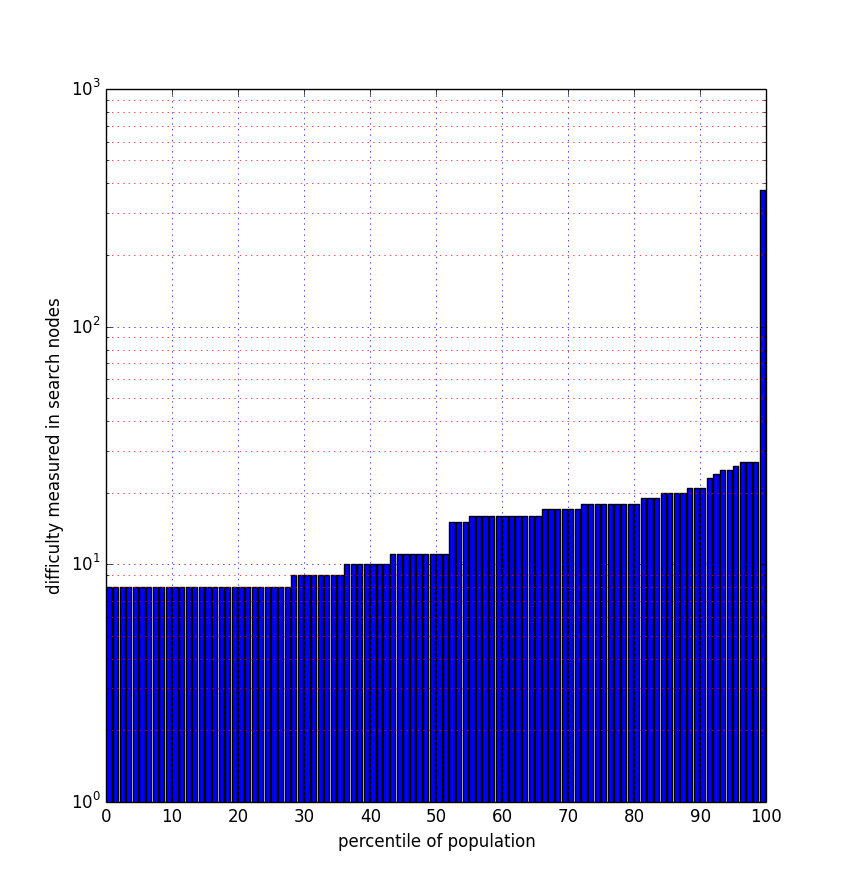
\includegraphics[height=11cm,width=9cm]{images/plots/pcmsSAT.png}
\end{minipage}%
\begin{minipage}[t]{.5\textwidth}
  \centering
  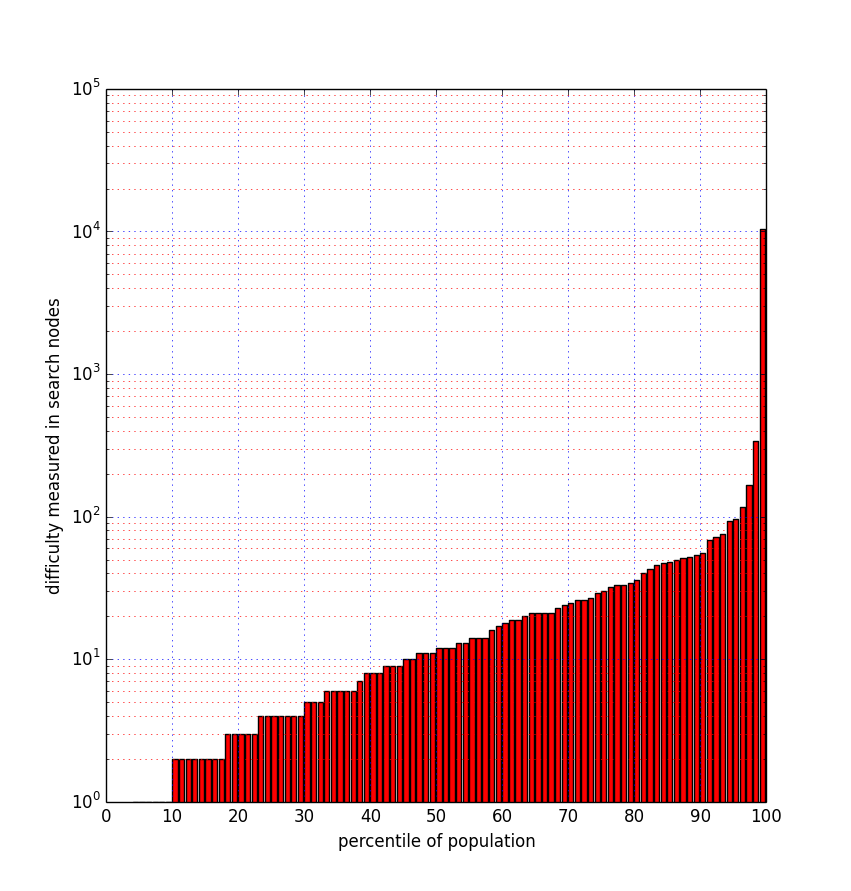
\includegraphics[height=11cm,width=9cm]{images/plots/pcmsUNSAT.png}
\end{minipage}
\caption{Search effort for \gls{sat}(blue, left) \gls{unsat}(red, right) \gls{sip} instances in pcms}
\label{fig:pcmsSatUnsat}
\end{figure}
\begin{figure}
\centering
\begin{minipage}[t]{.5\textwidth}
  \centering
  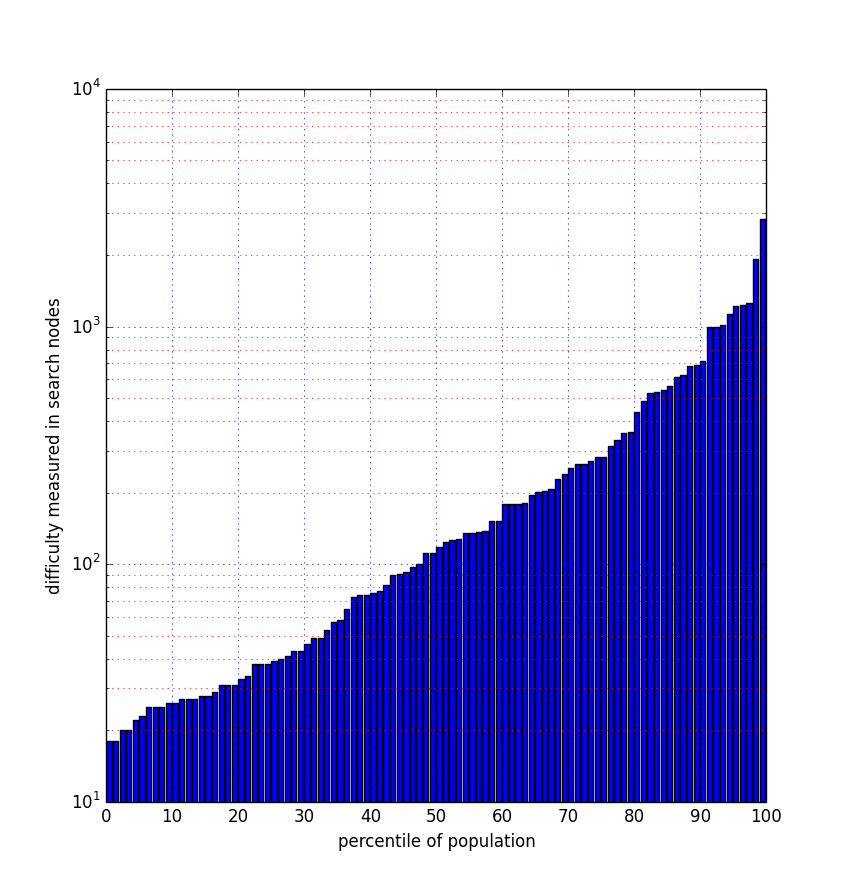
\includegraphics[height=11cm,width=9cm]{images/plots/pdbsSAT.png}
\end{minipage}%
\begin{minipage}[t]{.5\textwidth}
  \centering
  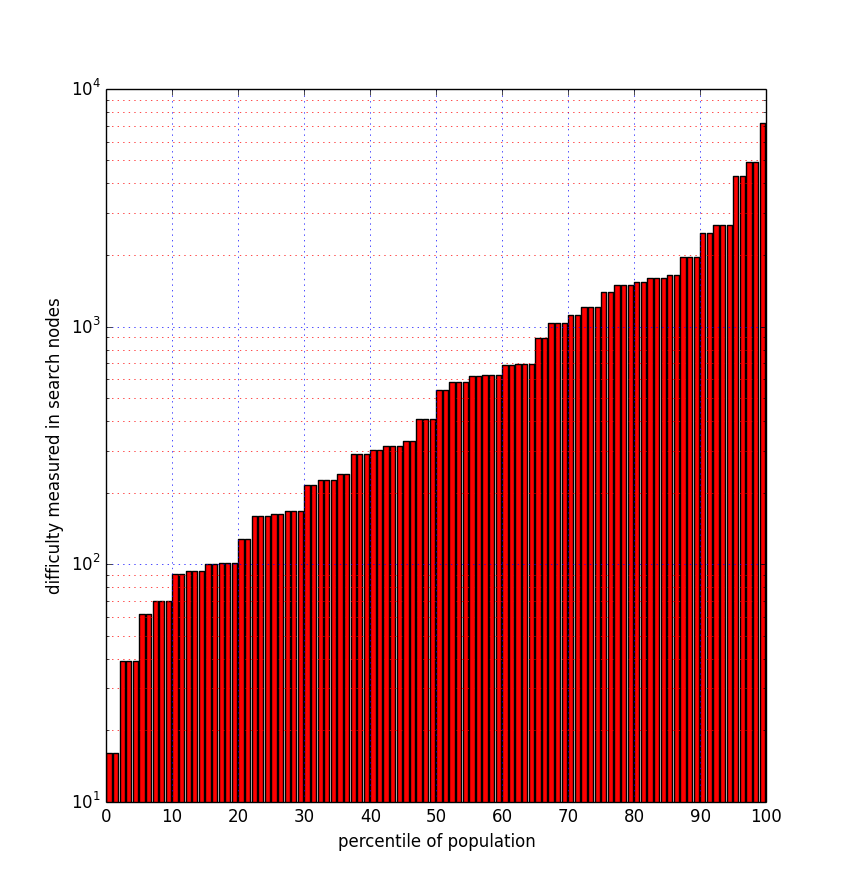
\includegraphics[height=11cm,width=9cm]{images/plots/pdbsUNSAT.png}
\end{minipage}
\caption{Search effort for \gls{sat}(blue, left) \gls{unsat}(red, right) \gls{sip} instances in pdbs}
\label{fig:pdbsSatUnsat}
\end{figure}
\begin{figure}
\centering
\begin{minipage}[t]{.5\textwidth}
  \centering
  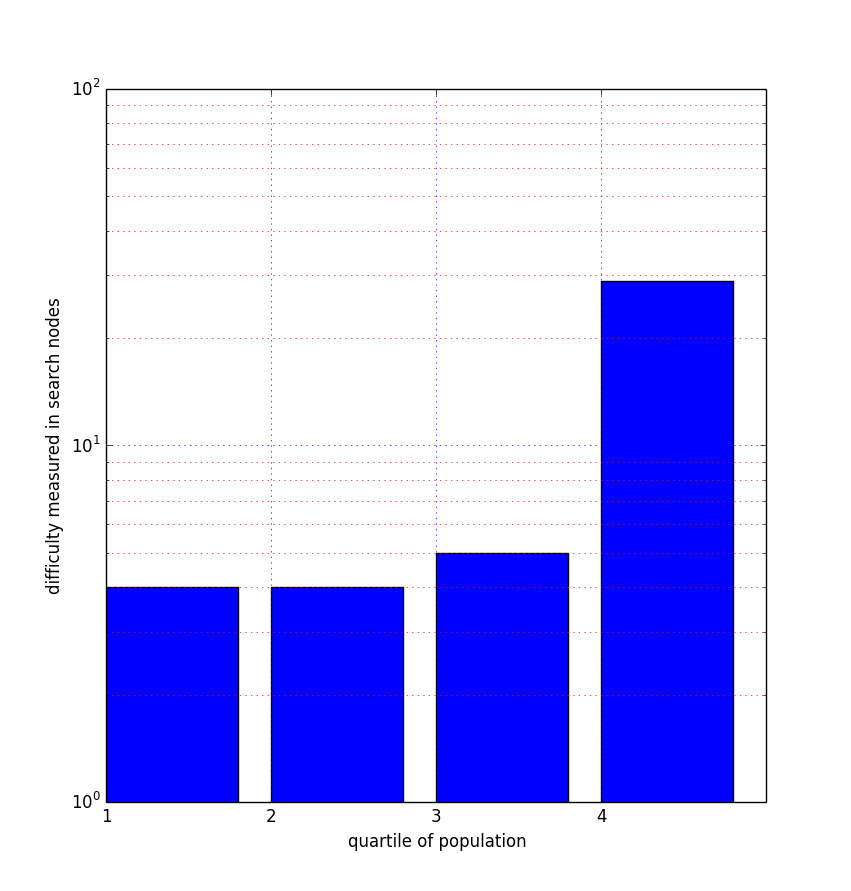
\includegraphics[height=11cm,width=9cm]{images/plots/ppigoSAT.png}
\end{minipage}%
\begin{minipage}[t]{.5\textwidth}
  \centering
  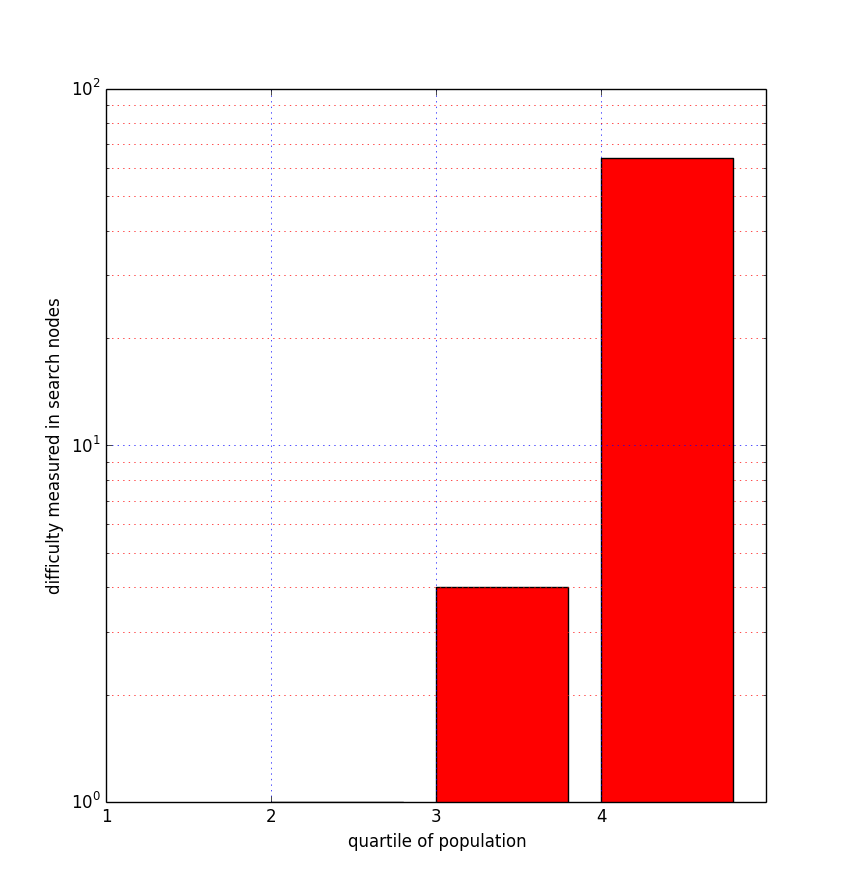
\includegraphics[height=11cm,width=9cm]{images/plots/ppigoUNSAT.png}
\end{minipage}
\caption{Search effort for \gls{sat}(blue, left) \gls{unsat}(red, right) \gls{sip} instances in ppigo}
\label{fig:ppigoSatUnsat}
\end{figure}
%%%%

Table \ref{table:SATUNSATnodes} presents statistics in terms of search effort for \gls{sat} (blue columns) and \gls{unsat} (red columns) instances. For instance, the Table shows that the total number of search nodes taken to solve all \gls{sat} \gls{sip} instances for the aids dataset is 437,108 and the total number of search nodes taken to solve all \gls{unsat} \gls{sip} instances in aids is 2,295,724. Using these Figures, we derive that the total number of search nodes taken to solve all \gls{sip} instances for the aids dataset is the sum of those two numbers, which is equal to 2,732,832. Figure \ref{table:dataSAT} shows the number of instances and percent from each category(SAT/UNSAT). The Table tells us that the reason for the large difference in terms of search effort between SAT and UNSAT instances is that 91\% of all instances are UNSAT (almost ten times more than SAT). Using the Tables and Figures, the following observations can be made:
\begin{itemize}
\item For aids, pcms and ppigo, the easiest percentile of \gls{unsat} \gls{sip} instances require less number of search nodes to be solved than the easiest \gls{sat} \gls{sip} instances. The hardest percentile of \gls{unsat} \gls{sip} take more search effort than the hardest percentile of \gls{sat} \gls{sip} instances.

\item For pdbs, there is a big difference in terms of search effort between SAT and UNSAT problems. For example, \gls{sat} instances are easier for every percentile of the targets (\ref{fig:pdbsSatUnsat}). The tabulated results on Figure \ref{table:SATUNSATnodes} confirm this observation. On average, SAT instances are 3 times easier than UNSAT, the SAT instances median is more than 4 times smaller than the UNSAT instances median and the number of search nodes taken to solve the hardest SAT instance (2,845) is much less than the number of nodes taken to solve the hardest UNSAT instance (7,152).

\item Table \ref{table:SATUNSATnodes} shows that for the pdbs dataset, the total search effort taken to solve unsatisfiable problems is bigger (894,260 nodes taken in total for SAT and 854,720 nodes in total taken for UNSAT problems) contrary to what we observed on the Figures. However, Table \ref{table:dataSAT} shows that \gls{sat} \gls{sip} consists of 77.22\% of all instances in pdbs. Therefore, the large search effort of SAT SIP problems for pdbs is due to their substantially larger number compared to UNSAT problems and in practice, \gls{unsat} \gls{sip} was much more difficult to solve than \gls{sat} \gls{sip} for this dataset. This is confirmed by the average search nodes figures (the second row in Table \ref{table:SATUNSATnodes}), where a SAT instance is on average 3 times easier to solve than an UNSAT instance.

\item The pcms dataset is composed of mostly \gls{unsat} \gls{sip} instances (\ref{table:dataSAT}, \ref{averageFailures}). Similarly to aids, this is the reason why the total number of search nodes for all \gls{unsat} problems is considerably larger than the number of search nodes for all \gls{sat} problems (\ref{table:SATUNSATnodes}). However, the hardest \gls{sat} problem is substantially easier than the hardest \gls{unsat}. The difference is 10,092 search nodes, where the SAT problem takes 378 search nodes to be solved (\ref{table:SATUNSATnodes}) and it is \gls{sip} (``\#32\_1CY1.cm.A.out'', ``\#1CY0.cm.A.cmap''), solved for 4 milliseconds. Average search nodes figures also show that a SAT instance is on average 5 times easier to solve than an UNSAT instance(the second row in Table \ref{table:SATUNSATnodes}).

\item 61\% of all instances in ppigo are \gls{sat} (\ref{table:dataSAT}, \ref{averageFailures}) and this is the main reason why the total SAT SIP search effort is larger than the UNSAT SIP search effort. The average search effort displayed in Table \ref{table:SATUNSATnodes} shows that SAT and UNSAT SIP instances are similarly hard on average for this dataset.
\end{itemize}


\newcolumntype{g}{>{\columncolor{red!15}}r}
\newcolumntype{b}{>{\columncolor{blue!15}}r}
\begin{table}
\centering
        \renewcommand{\arraystretch}{1.5}% Spread rows out...
        \begin{tabular}{c|bg|bg|bg|bg|bg|}
            \cline{2-11}
            &
             \multicolumn{2}{c}{\textbf{Total}} & 
             \multicolumn{2}{|c}{\textbf{Average}} & 
             \multicolumn{2}{|c|}{\textbf{Median}} & 
             \multicolumn{2}{c}{\textbf{Minimum}} & 
             \multicolumn{2}{|c|}{\textbf{Maximum}} \\
              \hline
            \cline{2-11}
             \hline
            % & SAT & UNSAT & SAT & UNSAT & SAT & UNSAT & SAT & UNSAT & SAT & UNSAT\\
            \multicolumn{1}{|c|}{\textbf{aids}}  &437,108  &2,295,724 &21 &10.4   &13  &0   &9  &0  &279   &619 \\
            \multicolumn{1}{|c|}{\textbf{pcms}}  &13,644   &133,276   &23 &110.3  &17  &9   &9  &0  &378   &10,470 \\
            \multicolumn{1}{|c|}{\textbf{pdbs}}  &894,260  &854,720   &322 &1,042.3 &123 &544 &18 &17 &2,845 &7,152 \\
            \multicolumn{1}{|c|}{\textbf{ppigo}} &714      &312       &6.932  &5.8    &6   &2   &5  &0  &30    &65 \\
            \hline
        \end{tabular}
        \caption{Number of nodes of search effort for each dataset. Blue for solvable and red for unsolvable SIP instances}
        \label{table:SATUNSATnodes}
    \end{table}


\subsection{Hardness of SIP in terms of running time}
Table \ref{table:cpuTime} shows the total time in milliseconds taken to solve all \gls{sip} instances of a given dataset. The time on the first row includes file I/O, creating and instantiating objects and domains of variables, the filtering and the verification time. The second row shows the number of milliseconds taken to perform the filtering step and the third: the \gls{sip} algorithm. Note that the filtering step is performed for every sip instance, whereas verification is applied only on instances that were not rejected during filtering. The percentage of calls to sip for each dataset can be seen on Figure \ref{table:failures}.

It is easy to notice that reading in the graphs from a file and instantiating the required objects and variables takes most of the running time for each dataset. For ppigo and pcms, filtering took more time than verification. These figures are very close for the aids dataset (filtering took 2,569 millis. and verification took 2,687 millis.). The 5,006 milliseconds spent on filtering for \gls{sip} problems in pdbs was wasteful, because no instance was rejected (\ref{averageFailures}). Performing \gls{sip} algorithm on all 3,600 instances (\ref{table:dataSAT}) took 16,102 milliseconds, which makes 4.47 milliseconds per instance on average. During the analysis of the search effort, it was noticed that pdbs is the hardest dataset. Achieving so fast verification time shows that the four Big Data datasets are indeed very easy.

\subsubsection{Comparison with Big Data algorithms}
\label{subsubsec:bigDataCompare}
Evaluation of six ``state of the art'' subgraph query processing algorithms (\cite{ctindex,gcode,GRAPES,tree+delta>=graph,graphgrepsx,freqStructBasedIndexing1}) is presented in \cite{foteini}. The algorithms employ a heavy filtering approach using an \gls{index} structure and run \cite{vf2} \gls{sip} algorithm during verification over the \gls{c}. We use the results in this work for comparison with the performance of the light filters method with the evaluated approaches.

In the study described in \cite{foteini}, it was observed that for pcms and ppigo, the filtering stage for four of the evaluated algorithms never finished executing, so the instances never underwent verification. Table \ref{table:cpuTime} shows that the performance of the light filters method is incomparably faster.

For the aids datasets, the fastest of the evaluated algorithms is GraphGrepSX \cite{graphgrepsx} and it took 9 seconds to perform filtering and about 600 milliseconds for verification. It took us 2,569 milliseconds for filtering (\ref{table:cpuTime}), but verification was slower (2,687 milliseconds). The fastest algorithm evaluated in \cite{foteini} took about 7 seconds for filtering and 200 milliseconds for verification and it is again GraphGrepSX \cite{graphgrepsx}. The light filters approach has slower verification and slightly faster filtering.

The algorithms evaluated in \cite{foteini} have an additional overhead that is not present in our approach, which is the size of the index that has to be stored.

\section{Summary of findings}
This Section includes a brief summary of the key points made in this Chapter. 

It was discovered that the Big Data datasets are of poor quality. Two of the datasets have targets that are copied multiple times each. All four datasets contain very easy \gls{sip} instances. The hardest of the datasets is pdbs. Even with the hardest dataset, a \gls{sip} instance took only 4.47 milliseconds to be solved on average. Verification for 50\% of the instances in pdbs took much less than 90 \glspl{sn}, the most expensive \gls{sip} problem costs 10,470 \glspl{sn}. Surprising finding was that the datasets can be easily kept in memory. Big Data is much smaller than what we initially expected. Beneficial future work in this area would be to develop better quality, much bigger and harder datasets. 

Filtering is bound to work only in the area of \gls{unsat} \gls{sip} instances. Consequently, when most of the instances of the dataset are \gls{sat}, filters can be more an overhead than help. The SIP algorithm, performed during verification, can both identify SAT and UNSAT problems. Therefore, constructing sophisticated filtering would give little gain, if any, but implementing fast and smart \gls{sip} would improve the performance significantly.  

We did experiments to find out whether \gls{sat} problems are generally easier than \gls{unsat} problems that were not rejected by filtering. What was observed is that for each of the datasets, the hardest and the easiest instances in terms of \glspl{sn} were \gls{unsat}. Possible way of improvement is to modify the filters algorithm so that it can prune those hard instances. This will involve further investigation of what makes a problem hard. 

\begin{table}
\centering
\renewcommand{\arraystretch}{1.3}% Spread rows out...
\begin{tabular}{ |>{\centering\bfseries}m{1.2in} |>{\centering}m{0.5in}| >{\centering}m{0.5in}| >{\centering}m{0.5in}| >{\centering\arraybackslash}m{0.5in}|} 
\hline
 & \textbf{AIDS} & \textbf{PCMS} & \textbf{PDBS}  & \textbf{PPIGO} \\
\hline
total cpu T & 15,770 & 26,855 & 133,451 & 11,886 \\
\hline
total filtering T & 2,569 & 1,500 & 5,006 & 379 \\
\hline
total verification T & 2,687 & 1,013 & 16,102 & 51 \\
\hline
\end{tabular}
\caption{Total running time in millisec for each dataset}
\label{table:cpuTime}
\end{table}    
   
\chapter{Conclusion and Future work}
	\section{What did we do? What does it suggest?}
    \section{Suggestions for Future work}

%%%%%%%%%%%%%%%%
%              %
%  APPENDICES  %
%              %
%%%%%%%%%%%%%%%%
\begin{appendices}

\chapter{Implementation}

%%%% table with query answers %%%%
\begin{table}[H]
\centering
\renewcommand{\arraystretch}{1.3}% Spread rows out...
\begin{tabular}{ >{\centering\bfseries}m{1in} >{\centering\arraybackslash}m{1.3in}  } 
\toprule
  Query Number & Answers Number\\
\midrule
 \textbf{0} &  8 042\\
 \rowcolor{Gray}
 \textbf{1} & 11 957\\
 \textbf{2} & 78\\
 \rowcolor{Gray}
 \textbf{3} & 461\\
 \textbf{4} & 77\\
  \rowcolor{Gray}
 \textbf{5} & 3\\ 
 \bottomrule
\end{tabular}
\caption{The number of answers for each query for aids dataset}
\label{table:answers}
\end{table}        
%%%%

An example of running from the command line is as follows:
\begin{verbatim}
      > java MaxClique BBMC1 brock200_1.clq 14400
\end{verbatim}
This will apply $BBMC$ with $style = 1$ to the first brock200 DIMACS instance allowing 14400 seconds of cpu time.

\chapter{Generating Random Graphs}
\label{sec:randomGraph}
We generate Erd\'{o}s-R\"{e}nyi random graphs $G(n,p)$ where $n$ is the number of vertices and
each edge is included in the graph with probability $p$ independent from every other edge. It produces
a random graph in DIMACS format with vertices numbered 1 to $n$ inclusive. It can be run from the command line as follows to produce 
a clq file
\begin{verbatim}
      > java RandomGraph 100 0.9 > 100-90-00.clq
\end{verbatim}
\end{appendices}

%%%%%%%%%%%%%%%%%%%%
%   BIBLIOGRAPHY   %
%%%%%%%%%%%%%%%%%%%%

\bibliographystyle{plain}
\bibliography{bib}
\printglossary
\printglossary[type=\acronymtype]
\end{document}
